% Created by tikzDevice version 0.12.3.1 on 2022-04-15 21:34:04
% !TEX encoding = UTF-8 Unicode
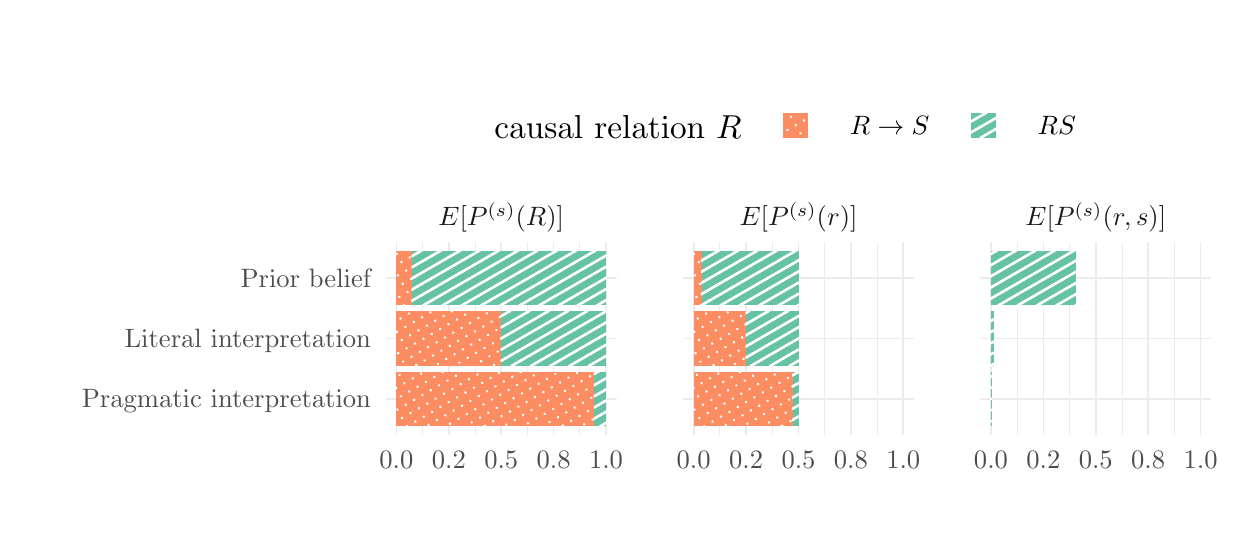
\begin{tikzpicture}[x=1pt,y=1pt]
\definecolor{fillColor}{RGB}{255,255,255}
\path[use as bounding box,fill=fillColor,fill opacity=0.00] (0,0) rectangle (433.62,180.67);
\begin{scope}
\path[clip] (129.45, 33.48) rectangle (212.78,103.28);
\definecolor{drawColor}{gray}{0.92}

\path[draw=drawColor,line width= 0.3pt,line join=round] (142.71, 33.48) --
	(142.71,103.28);

\path[draw=drawColor,line width= 0.3pt,line join=round] (161.65, 33.48) --
	(161.65,103.28);

\path[draw=drawColor,line width= 0.3pt,line join=round] (180.59, 33.48) --
	(180.59,103.28);

\path[draw=drawColor,line width= 0.3pt,line join=round] (199.52, 33.48) --
	(199.52,103.28);

\path[draw=drawColor,line width= 0.6pt,line join=round] (129.45, 46.56) --
	(212.78, 46.56);

\path[draw=drawColor,line width= 0.6pt,line join=round] (129.45, 68.38) --
	(212.78, 68.38);

\path[draw=drawColor,line width= 0.6pt,line join=round] (129.45, 90.19) --
	(212.78, 90.19);

\path[draw=drawColor,line width= 0.6pt,line join=round] (133.24, 33.48) --
	(133.24,103.28);

\path[draw=drawColor,line width= 0.6pt,line join=round] (152.18, 33.48) --
	(152.18,103.28);

\path[draw=drawColor,line width= 0.6pt,line join=round] (171.12, 33.48) --
	(171.12,103.28);

\path[draw=drawColor,line width= 0.6pt,line join=round] (190.06, 33.48) --
	(190.06,103.28);

\path[draw=drawColor,line width= 0.6pt,line join=round] (208.99, 33.48) --
	(208.99,103.28);
\definecolor{fillColor}{RGB}{102,194,165}

\path[fill=fillColor] (204.79, 36.75) rectangle (208.99, 56.38);
\definecolor{fillColor}{RGB}{252,141,98}

\path[fill=fillColor] (133.24, 36.75) rectangle (204.79, 56.38);
\definecolor{fillColor}{RGB}{102,194,165}

\path[fill=fillColor] (171.12, 58.56) rectangle (208.99, 78.20);
\definecolor{fillColor}{RGB}{252,141,98}

\path[fill=fillColor] (133.24, 58.56) rectangle (171.12, 78.20);

\path[fill=fillColor] (133.24, 80.38) rectangle (138.92,100.01);
\definecolor{fillColor}{RGB}{102,194,165}

\path[fill=fillColor] (138.92, 80.38) rectangle (203.31,100.01);

\path[fill=fillColor] (203.31, 80.38) rectangle (208.99,100.01);
\definecolor{drawColor}{RGB}{255,255,255}
\definecolor{fillColor}{RGB}{255,255,255}

\path[draw=drawColor,line width= 0.6pt,line join=round,line cap=rect,fill=fillColor] (206.73, 36.75) --
	(208.99, 38.05) --
	(208.99, 37.65) --
	(207.43, 36.75) --
	(206.73, 36.75) --
	cycle;

\path[draw=drawColor,line width= 0.6pt,line join=round,line cap=rect,fill=fillColor] (204.79, 39.65) --
	(208.99, 42.08) --
	(208.99, 41.68) --
	(204.79, 39.25) --
	(204.79, 39.65) --
	cycle;

\path[draw=drawColor,line width= 0.6pt,line join=round,line cap=rect,fill=fillColor] (204.79, 43.69) --
	(208.99, 46.12) --
	(208.99, 45.71) --
	(204.79, 43.28) --
	(204.79, 43.69) --
	cycle;

\path[draw=drawColor,line width= 0.6pt,line join=round,line cap=rect,fill=fillColor] (204.79, 47.72) --
	(208.99, 50.15) --
	(208.99, 49.74) --
	(204.79, 47.31) --
	(204.79, 47.72) --
	cycle;

\path[draw=drawColor,line width= 0.6pt,line join=round,line cap=rect,fill=fillColor] (204.79, 51.75) --
	(208.99, 54.18) --
	(208.99, 53.77) --
	(204.79, 51.34) --
	(204.79, 51.75) --
	cycle;

\path[draw=drawColor,line width= 0.6pt,line join=round,line cap=rect,fill=fillColor] (204.79, 55.78) --
	(205.83, 56.38) --
	(206.53, 56.38) --
	(204.79, 55.37) --
	(204.79, 55.78) --
	cycle;

\path[draw=drawColor,line width= 0.6pt,dash pattern=on 2pt off 2pt ,line join=round,line cap=round,fill=fillColor] (133.57, 42.67) circle (  0.17);

\path[draw=drawColor,line width= 0.6pt,dash pattern=on 2pt off 2pt ,line join=round,line cap=round,fill=fillColor] (134.38, 55.23) circle (  0.17);

\path[draw=drawColor,line width= 0.6pt,dash pattern=on 2pt off 2pt ,line join=round,line cap=round,fill=fillColor] (134.84, 47.44) circle (  0.17);

\path[draw=drawColor,line width= 0.6pt,dash pattern=on 2pt off 2pt ,line join=round,line cap=round,fill=fillColor] (135.31, 39.65) circle (  0.17);

\path[draw=drawColor,line width= 0.6pt,dash pattern=on 2pt off 2pt ,line join=round,line cap=round,fill=fillColor] (136.12, 52.20) circle (  0.17);

\path[draw=drawColor,line width= 0.6pt,dash pattern=on 2pt off 2pt ,line join=round,line cap=round,fill=fillColor] (136.59, 44.41) circle (  0.17);

\path[draw=drawColor,line width= 0.6pt,dash pattern=on 2pt off 2pt ,line join=round,line cap=round,fill=fillColor] (137.87, 49.18) circle (  0.17);

\path[draw=drawColor,line width= 0.6pt,dash pattern=on 2pt off 2pt ,line join=round,line cap=round,fill=fillColor] (138.33, 41.39) circle (  0.17);

\path[draw=drawColor,line width= 0.6pt,dash pattern=on 2pt off 2pt ,line join=round,line cap=round,fill=fillColor] (139.14, 53.95) circle (  0.17);

\path[draw=drawColor,line width= 0.6pt,dash pattern=on 2pt off 2pt ,line join=round,line cap=round,fill=fillColor] (139.61, 46.16) circle (  0.17);

\path[draw=drawColor,line width= 0.6pt,dash pattern=on 2pt off 2pt ,line join=round,line cap=round,fill=fillColor] (140.08, 38.37) circle (  0.17);

\path[draw=drawColor,line width= 0.6pt,dash pattern=on 2pt off 2pt ,line join=round,line cap=round,fill=fillColor] (140.89, 50.93) circle (  0.17);

\path[draw=drawColor,line width= 0.6pt,dash pattern=on 2pt off 2pt ,line join=round,line cap=round,fill=fillColor] (141.36, 43.14) circle (  0.17);

\path[draw=drawColor,line width= 0.6pt,dash pattern=on 2pt off 2pt ,line join=round,line cap=round,fill=fillColor] (142.17, 55.70) circle (  0.17);

\path[draw=drawColor,line width= 0.6pt,dash pattern=on 2pt off 2pt ,line join=round,line cap=round,fill=fillColor] (142.63, 47.90) circle (  0.17);

\path[draw=drawColor,line width= 0.6pt,dash pattern=on 2pt off 2pt ,line join=round,line cap=round,fill=fillColor] (143.10, 40.11) circle (  0.17);

\path[draw=drawColor,line width= 0.6pt,dash pattern=on 2pt off 2pt ,line join=round,line cap=round,fill=fillColor] (143.91, 52.67) circle (  0.17);

\path[draw=drawColor,line width= 0.6pt,dash pattern=on 2pt off 2pt ,line join=round,line cap=round,fill=fillColor] (144.38, 44.88) circle (  0.17);

\path[draw=drawColor,line width= 0.6pt,dash pattern=on 2pt off 2pt ,line join=round,line cap=round,fill=fillColor] (144.85, 37.09) circle (  0.17);

\path[draw=drawColor,line width= 0.6pt,dash pattern=on 2pt off 2pt ,line join=round,line cap=round,fill=fillColor] (145.66, 49.65) circle (  0.17);

\path[draw=drawColor,line width= 0.6pt,dash pattern=on 2pt off 2pt ,line join=round,line cap=round,fill=fillColor] (146.13, 41.86) circle (  0.17);

\path[draw=drawColor,line width= 0.6pt,dash pattern=on 2pt off 2pt ,line join=round,line cap=round,fill=fillColor] (146.94, 54.42) circle (  0.17);

\path[draw=drawColor,line width= 0.6pt,dash pattern=on 2pt off 2pt ,line join=round,line cap=round,fill=fillColor] (147.40, 46.63) circle (  0.17);

\path[draw=drawColor,line width= 0.6pt,dash pattern=on 2pt off 2pt ,line join=round,line cap=round,fill=fillColor] (147.87, 38.84) circle (  0.17);

\path[draw=drawColor,line width= 0.6pt,dash pattern=on 2pt off 2pt ,line join=round,line cap=round,fill=fillColor] (148.68, 51.39) circle (  0.17);

\path[draw=drawColor,line width= 0.6pt,dash pattern=on 2pt off 2pt ,line join=round,line cap=round,fill=fillColor] (149.15, 43.60) circle (  0.17);

\path[draw=drawColor,line width= 0.6pt,dash pattern=on 2pt off 2pt ,line join=round,line cap=round,fill=fillColor] (149.96, 56.16) circle (  0.17);

\path[draw=drawColor,line width= 0.6pt,dash pattern=on 2pt off 2pt ,line join=round,line cap=round,fill=fillColor] (150.43, 48.37) circle (  0.17);

\path[draw=drawColor,line width= 0.6pt,dash pattern=on 2pt off 2pt ,line join=round,line cap=round,fill=fillColor] (150.89, 40.58) circle (  0.17);

\path[draw=drawColor,line width= 0.6pt,dash pattern=on 2pt off 2pt ,line join=round,line cap=round,fill=fillColor] (151.70, 53.14) circle (  0.17);

\path[draw=drawColor,line width= 0.6pt,dash pattern=on 2pt off 2pt ,line join=round,line cap=round,fill=fillColor] (152.17, 45.35) circle (  0.17);

\path[draw=drawColor,line width= 0.6pt,dash pattern=on 2pt off 2pt ,line join=round,line cap=round,fill=fillColor] (152.64, 37.56) circle (  0.17);

\path[draw=drawColor,line width= 0.6pt,dash pattern=on 2pt off 2pt ,line join=round,line cap=round,fill=fillColor] (153.45, 50.12) circle (  0.17);

\path[draw=drawColor,line width= 0.6pt,dash pattern=on 2pt off 2pt ,line join=round,line cap=round,fill=fillColor] (153.92, 42.33) circle (  0.17);

\path[draw=drawColor,line width= 0.6pt,dash pattern=on 2pt off 2pt ,line join=round,line cap=round,fill=fillColor] (154.73, 54.89) circle (  0.17);

\path[draw=drawColor,line width= 0.6pt,dash pattern=on 2pt off 2pt ,line join=round,line cap=round,fill=fillColor] (155.19, 47.09) circle (  0.17);

\path[draw=drawColor,line width= 0.6pt,dash pattern=on 2pt off 2pt ,line join=round,line cap=round,fill=fillColor] (155.66, 39.30) circle (  0.17);

\path[draw=drawColor,line width= 0.6pt,dash pattern=on 2pt off 2pt ,line join=round,line cap=round,fill=fillColor] (156.47, 51.86) circle (  0.17);

\path[draw=drawColor,line width= 0.6pt,dash pattern=on 2pt off 2pt ,line join=round,line cap=round,fill=fillColor] (156.94, 44.07) circle (  0.17);

\path[draw=drawColor,line width= 0.6pt,dash pattern=on 2pt off 2pt ,line join=round,line cap=round,fill=fillColor] (158.22, 48.84) circle (  0.17);

\path[draw=drawColor,line width= 0.6pt,dash pattern=on 2pt off 2pt ,line join=round,line cap=round,fill=fillColor] (158.68, 41.05) circle (  0.17);

\path[draw=drawColor,line width= 0.6pt,dash pattern=on 2pt off 2pt ,line join=round,line cap=round,fill=fillColor] (159.49, 53.61) circle (  0.17);

\path[draw=drawColor,line width= 0.6pt,dash pattern=on 2pt off 2pt ,line join=round,line cap=round,fill=fillColor] (159.96, 45.82) circle (  0.17);

\path[draw=drawColor,line width= 0.6pt,dash pattern=on 2pt off 2pt ,line join=round,line cap=round,fill=fillColor] (160.43, 38.03) circle (  0.17);

\path[draw=drawColor,line width= 0.6pt,dash pattern=on 2pt off 2pt ,line join=round,line cap=round,fill=fillColor] (161.24, 50.58) circle (  0.17);

\path[draw=drawColor,line width= 0.6pt,dash pattern=on 2pt off 2pt ,line join=round,line cap=round,fill=fillColor] (161.71, 42.79) circle (  0.17);

\path[draw=drawColor,line width= 0.6pt,dash pattern=on 2pt off 2pt ,line join=round,line cap=round,fill=fillColor] (162.52, 55.35) circle (  0.17);

\path[draw=drawColor,line width= 0.6pt,dash pattern=on 2pt off 2pt ,line join=round,line cap=round,fill=fillColor] (162.98, 47.56) circle (  0.17);

\path[draw=drawColor,line width= 0.6pt,dash pattern=on 2pt off 2pt ,line join=round,line cap=round,fill=fillColor] (163.45, 39.77) circle (  0.17);

\path[draw=drawColor,line width= 0.6pt,dash pattern=on 2pt off 2pt ,line join=round,line cap=round,fill=fillColor] (164.26, 52.33) circle (  0.17);

\path[draw=drawColor,line width= 0.6pt,dash pattern=on 2pt off 2pt ,line join=round,line cap=round,fill=fillColor] (164.73, 44.54) circle (  0.17);

\path[draw=drawColor,line width= 0.6pt,dash pattern=on 2pt off 2pt ,line join=round,line cap=round,fill=fillColor] (166.01, 49.31) circle (  0.17);

\path[draw=drawColor,line width= 0.6pt,dash pattern=on 2pt off 2pt ,line join=round,line cap=round,fill=fillColor] (166.47, 41.52) circle (  0.17);

\path[draw=drawColor,line width= 0.6pt,dash pattern=on 2pt off 2pt ,line join=round,line cap=round,fill=fillColor] (167.28, 54.08) circle (  0.17);

\path[draw=drawColor,line width= 0.6pt,dash pattern=on 2pt off 2pt ,line join=round,line cap=round,fill=fillColor] (167.75, 46.28) circle (  0.17);

\path[draw=drawColor,line width= 0.6pt,dash pattern=on 2pt off 2pt ,line join=round,line cap=round,fill=fillColor] (168.22, 38.49) circle (  0.17);

\path[draw=drawColor,line width= 0.6pt,dash pattern=on 2pt off 2pt ,line join=round,line cap=round,fill=fillColor] (169.03, 51.05) circle (  0.17);

\path[draw=drawColor,line width= 0.6pt,dash pattern=on 2pt off 2pt ,line join=round,line cap=round,fill=fillColor] (169.50, 43.26) circle (  0.17);

\path[draw=drawColor,line width= 0.6pt,dash pattern=on 2pt off 2pt ,line join=round,line cap=round,fill=fillColor] (170.31, 55.82) circle (  0.17);

\path[draw=drawColor,line width= 0.6pt,dash pattern=on 2pt off 2pt ,line join=round,line cap=round,fill=fillColor] (170.77, 48.03) circle (  0.17);

\path[draw=drawColor,line width= 0.6pt,dash pattern=on 2pt off 2pt ,line join=round,line cap=round,fill=fillColor] (171.24, 40.24) circle (  0.17);

\path[draw=drawColor,line width= 0.6pt,dash pattern=on 2pt off 2pt ,line join=round,line cap=round,fill=fillColor] (172.05, 52.80) circle (  0.17);

\path[draw=drawColor,line width= 0.6pt,dash pattern=on 2pt off 2pt ,line join=round,line cap=round,fill=fillColor] (172.52, 45.01) circle (  0.17);

\path[draw=drawColor,line width= 0.6pt,dash pattern=on 2pt off 2pt ,line join=round,line cap=round,fill=fillColor] (172.99, 37.22) circle (  0.17);

\path[draw=drawColor,line width= 0.6pt,dash pattern=on 2pt off 2pt ,line join=round,line cap=round,fill=fillColor] (173.80, 49.77) circle (  0.17);

\path[draw=drawColor,line width= 0.6pt,dash pattern=on 2pt off 2pt ,line join=round,line cap=round,fill=fillColor] (174.27, 41.98) circle (  0.17);

\path[draw=drawColor,line width= 0.6pt,dash pattern=on 2pt off 2pt ,line join=round,line cap=round,fill=fillColor] (175.08, 54.54) circle (  0.17);

\path[draw=drawColor,line width= 0.6pt,dash pattern=on 2pt off 2pt ,line join=round,line cap=round,fill=fillColor] (175.54, 46.75) circle (  0.17);

\path[draw=drawColor,line width= 0.6pt,dash pattern=on 2pt off 2pt ,line join=round,line cap=round,fill=fillColor] (176.01, 38.96) circle (  0.17);

\path[draw=drawColor,line width= 0.6pt,dash pattern=on 2pt off 2pt ,line join=round,line cap=round,fill=fillColor] (176.82, 51.52) circle (  0.17);

\path[draw=drawColor,line width= 0.6pt,dash pattern=on 2pt off 2pt ,line join=round,line cap=round,fill=fillColor] (177.29, 43.73) circle (  0.17);

\path[draw=drawColor,line width= 0.6pt,dash pattern=on 2pt off 2pt ,line join=round,line cap=round,fill=fillColor] (178.57, 48.50) circle (  0.17);

\path[draw=drawColor,line width= 0.6pt,dash pattern=on 2pt off 2pt ,line join=round,line cap=round,fill=fillColor] (179.03, 40.71) circle (  0.17);

\path[draw=drawColor,line width= 0.6pt,dash pattern=on 2pt off 2pt ,line join=round,line cap=round,fill=fillColor] (179.84, 53.27) circle (  0.17);

\path[draw=drawColor,line width= 0.6pt,dash pattern=on 2pt off 2pt ,line join=round,line cap=round,fill=fillColor] (180.31, 45.47) circle (  0.17);

\path[draw=drawColor,line width= 0.6pt,dash pattern=on 2pt off 2pt ,line join=round,line cap=round,fill=fillColor] (180.78, 37.68) circle (  0.17);

\path[draw=drawColor,line width= 0.6pt,dash pattern=on 2pt off 2pt ,line join=round,line cap=round,fill=fillColor] (181.59, 50.24) circle (  0.17);

\path[draw=drawColor,line width= 0.6pt,dash pattern=on 2pt off 2pt ,line join=round,line cap=round,fill=fillColor] (182.06, 42.45) circle (  0.17);

\path[draw=drawColor,line width= 0.6pt,dash pattern=on 2pt off 2pt ,line join=round,line cap=round,fill=fillColor] (182.87, 55.01) circle (  0.17);

\path[draw=drawColor,line width= 0.6pt,dash pattern=on 2pt off 2pt ,line join=round,line cap=round,fill=fillColor] (183.33, 47.22) circle (  0.17);

\path[draw=drawColor,line width= 0.6pt,dash pattern=on 2pt off 2pt ,line join=round,line cap=round,fill=fillColor] (183.80, 39.43) circle (  0.17);

\path[draw=drawColor,line width= 0.6pt,dash pattern=on 2pt off 2pt ,line join=round,line cap=round,fill=fillColor] (184.61, 51.99) circle (  0.17);

\path[draw=drawColor,line width= 0.6pt,dash pattern=on 2pt off 2pt ,line join=round,line cap=round,fill=fillColor] (185.08, 44.20) circle (  0.17);

\path[draw=drawColor,line width= 0.6pt,dash pattern=on 2pt off 2pt ,line join=round,line cap=round,fill=fillColor] (186.36, 48.96) circle (  0.17);

\path[draw=drawColor,line width= 0.6pt,dash pattern=on 2pt off 2pt ,line join=round,line cap=round,fill=fillColor] (186.82, 41.17) circle (  0.17);

\path[draw=drawColor,line width= 0.6pt,dash pattern=on 2pt off 2pt ,line join=round,line cap=round,fill=fillColor] (187.63, 53.73) circle (  0.17);

\path[draw=drawColor,line width= 0.6pt,dash pattern=on 2pt off 2pt ,line join=round,line cap=round,fill=fillColor] (188.10, 45.94) circle (  0.17);

\path[draw=drawColor,line width= 0.6pt,dash pattern=on 2pt off 2pt ,line join=round,line cap=round,fill=fillColor] (188.57, 38.15) circle (  0.17);

\path[draw=drawColor,line width= 0.6pt,dash pattern=on 2pt off 2pt ,line join=round,line cap=round,fill=fillColor] (189.38, 50.71) circle (  0.17);

\path[draw=drawColor,line width= 0.6pt,dash pattern=on 2pt off 2pt ,line join=round,line cap=round,fill=fillColor] (189.85, 42.92) circle (  0.17);

\path[draw=drawColor,line width= 0.6pt,dash pattern=on 2pt off 2pt ,line join=round,line cap=round,fill=fillColor] (190.66, 55.48) circle (  0.17);

\path[draw=drawColor,line width= 0.6pt,dash pattern=on 2pt off 2pt ,line join=round,line cap=round,fill=fillColor] (191.12, 47.69) circle (  0.17);

\path[draw=drawColor,line width= 0.6pt,dash pattern=on 2pt off 2pt ,line join=round,line cap=round,fill=fillColor] (191.59, 39.90) circle (  0.17);

\path[draw=drawColor,line width= 0.6pt,dash pattern=on 2pt off 2pt ,line join=round,line cap=round,fill=fillColor] (192.40, 52.46) circle (  0.17);

\path[draw=drawColor,line width= 0.6pt,dash pattern=on 2pt off 2pt ,line join=round,line cap=round,fill=fillColor] (192.87, 44.66) circle (  0.17);

\path[draw=drawColor,line width= 0.6pt,dash pattern=on 2pt off 2pt ,line join=round,line cap=round,fill=fillColor] (194.15, 49.43) circle (  0.17);

\path[draw=drawColor,line width= 0.6pt,dash pattern=on 2pt off 2pt ,line join=round,line cap=round,fill=fillColor] (194.61, 41.64) circle (  0.17);

\path[draw=drawColor,line width= 0.6pt,dash pattern=on 2pt off 2pt ,line join=round,line cap=round,fill=fillColor] (195.42, 54.20) circle (  0.17);

\path[draw=drawColor,line width= 0.6pt,dash pattern=on 2pt off 2pt ,line join=round,line cap=round,fill=fillColor] (195.89, 46.41) circle (  0.17);

\path[draw=drawColor,line width= 0.6pt,dash pattern=on 2pt off 2pt ,line join=round,line cap=round,fill=fillColor] (196.36, 38.62) circle (  0.17);

\path[draw=drawColor,line width= 0.6pt,dash pattern=on 2pt off 2pt ,line join=round,line cap=round,fill=fillColor] (197.17, 51.18) circle (  0.17);

\path[draw=drawColor,line width= 0.6pt,dash pattern=on 2pt off 2pt ,line join=round,line cap=round,fill=fillColor] (197.64, 43.39) circle (  0.17);

\path[draw=drawColor,line width= 0.6pt,dash pattern=on 2pt off 2pt ,line join=round,line cap=round,fill=fillColor] (198.45, 55.95) circle (  0.17);

\path[draw=drawColor,line width= 0.6pt,dash pattern=on 2pt off 2pt ,line join=round,line cap=round,fill=fillColor] (198.91, 48.16) circle (  0.17);

\path[draw=drawColor,line width= 0.6pt,dash pattern=on 2pt off 2pt ,line join=round,line cap=round,fill=fillColor] (199.38, 40.36) circle (  0.17);

\path[draw=drawColor,line width= 0.6pt,dash pattern=on 2pt off 2pt ,line join=round,line cap=round,fill=fillColor] (200.19, 52.92) circle (  0.17);

\path[draw=drawColor,line width= 0.6pt,dash pattern=on 2pt off 2pt ,line join=round,line cap=round,fill=fillColor] (200.66, 45.13) circle (  0.17);

\path[draw=drawColor,line width= 0.6pt,dash pattern=on 2pt off 2pt ,line join=round,line cap=round,fill=fillColor] (201.13, 37.34) circle (  0.17);

\path[draw=drawColor,line width= 0.6pt,dash pattern=on 2pt off 2pt ,line join=round,line cap=round,fill=fillColor] (201.94, 49.90) circle (  0.17);

\path[draw=drawColor,line width= 0.6pt,dash pattern=on 2pt off 2pt ,line join=round,line cap=round,fill=fillColor] (202.41, 42.11) circle (  0.17);

\path[draw=drawColor,line width= 0.6pt,dash pattern=on 2pt off 2pt ,line join=round,line cap=round,fill=fillColor] (203.22, 54.67) circle (  0.17);

\path[draw=drawColor,line width= 0.6pt,dash pattern=on 2pt off 2pt ,line join=round,line cap=round,fill=fillColor] (203.68, 46.88) circle (  0.17);

\path[draw=drawColor,line width= 0.6pt,dash pattern=on 2pt off 2pt ,line join=round,line cap=round,fill=fillColor] (204.15, 39.09) circle (  0.17);

\path[draw=drawColor,line width= 0.6pt,dash pattern=on 2pt off 2pt ,line join=round,line cap=round,fill=fillColor] (133.24, 50.56) --
	(133.24, 50.56) --
	(133.25, 50.55) --
	(133.26, 50.54) --
	(133.26, 50.53) --
	(133.26, 50.52) --
	(133.27, 50.51) --
	(133.27, 50.50) --
	(133.27, 50.49) --
	(133.27, 50.47) --
	(133.27, 50.46) --
	(133.27, 50.45) --
	(133.27, 50.44) --
	(133.27, 50.43) --
	(133.27, 50.42) --
	(133.27, 50.41) --
	(133.26, 50.40) --
	(133.26, 50.39) --
	(133.25, 50.38) --
	(133.25, 50.37) --
	(133.24, 50.36) --
	(133.24, 50.36) --
	(133.24, 50.56) --
	cycle;

\path[draw=drawColor,line width= 0.6pt,dash pattern=on 2pt off 2pt ,line join=round,line cap=round,fill=fillColor] (136.93, 36.75) --
	(136.93, 36.75) --
	(136.94, 36.76) --
	(136.95, 36.76) --
	(136.96, 36.77) --
	(136.97, 36.77) --
	(136.98, 36.78) --
	(136.99, 36.78) --
	(137.00, 36.79) --
	(137.01, 36.79) --
	(137.02, 36.79) --
	(137.03, 36.80) --
	(137.04, 36.80) --
	(137.05, 36.80) --
	(137.06, 36.80) --
	(137.08, 36.80) --
	(137.09, 36.80) --
	(137.10, 36.79) --
	(137.11, 36.79) --
	(137.12, 36.79) --
	(137.13, 36.78) --
	(137.14, 36.78) --
	(137.15, 36.77) --
	(137.16, 36.77) --
	(137.17, 36.76) --
	(137.17, 36.75) --
	(137.18, 36.75) --
	(136.93, 36.75) --
	cycle;

\path[draw=drawColor,line width= 0.6pt,dash pattern=on 2pt off 2pt ,line join=round,line cap=round,fill=fillColor] (165.02, 36.75) --
	(165.02, 36.76) --
	(165.02, 36.77) --
	(165.02, 36.78) --
	(165.03, 36.79) --
	(165.03, 36.80) --
	(165.03, 36.81) --
	(165.04, 36.82) --
	(165.04, 36.83) --
	(165.05, 36.84) --
	(165.05, 36.85) --
	(165.06, 36.86) --
	(165.07, 36.87) --
	(165.07, 36.87) --
	(165.08, 36.88) --
	(165.09, 36.89) --
	(165.10, 36.89) --
	(165.11, 36.90) --
	(165.12, 36.91) --
	(165.13, 36.91) --
	(165.14, 36.91) --
	(165.15, 36.92) --
	(165.16, 36.92) --
	(165.17, 36.92) --
	(165.18, 36.92) --
	(165.19, 36.92) --
	(165.20, 36.92) --
	(165.22, 36.92) --
	(165.23, 36.92) --
	(165.24, 36.92) --
	(165.25, 36.92) --
	(165.26, 36.91) --
	(165.27, 36.91) --
	(165.28, 36.90) --
	(165.29, 36.90) --
	(165.30, 36.89) --
	(165.31, 36.89) --
	(165.31, 36.88) --
	(165.32, 36.87) --
	(165.33, 36.86) --
	(165.34, 36.85) --
	(165.34, 36.85) --
	(165.35, 36.84) --
	(165.35, 36.83) --
	(165.36, 36.82) --
	(165.36, 36.81) --
	(165.37, 36.80) --
	(165.37, 36.78) --
	(165.37, 36.77) --
	(165.37, 36.76) --
	(165.37, 36.75) --
	(165.37, 36.75) --
	(165.02, 36.75) --
	cycle;

\path[draw=drawColor,line width= 0.6pt,dash pattern=on 2pt off 2pt ,line join=round,line cap=round,fill=fillColor] (178.25, 56.38) --
	(178.25, 56.38) --
	(178.25, 56.37) --
	(178.26, 56.36) --
	(178.26, 56.35) --
	(178.27, 56.33) --
	(178.27, 56.32) --
	(178.27, 56.31) --
	(178.27, 56.30) --
	(178.27, 56.29) --
	(178.27, 56.28) --
	(178.27, 56.27) --
	(178.27, 56.26) --
	(178.27, 56.25) --
	(178.26, 56.24) --
	(178.26, 56.23) --
	(178.26, 56.22) --
	(178.25, 56.21) --
	(178.25, 56.20) --
	(178.24, 56.19) --
	(178.23, 56.18) --
	(178.23, 56.17) --
	(178.22, 56.16) --
	(178.21, 56.16) --
	(178.20, 56.15) --
	(178.19, 56.14) --
	(178.19, 56.14) --
	(178.18, 56.13) --
	(178.17, 56.13) --
	(178.16, 56.12) --
	(178.14, 56.12) --
	(178.13, 56.12) --
	(178.12, 56.12) --
	(178.11, 56.11) --
	(178.10, 56.11) --
	(178.09, 56.11) --
	(178.08, 56.11) --
	(178.07, 56.12) --
	(178.06, 56.12) --
	(178.05, 56.12) --
	(178.04, 56.12) --
	(178.03, 56.13) --
	(178.02, 56.13) --
	(178.01, 56.14) --
	(178.00, 56.14) --
	(177.99, 56.15) --
	(177.98, 56.16) --
	(177.97, 56.17) --
	(177.97, 56.17) --
	(177.96, 56.18) --
	(177.95, 56.19) --
	(177.95, 56.20) --
	(177.94, 56.21) --
	(177.94, 56.22) --
	(177.93, 56.23) --
	(177.93, 56.24) --
	(177.93, 56.25) --
	(177.93, 56.26) --
	(177.92, 56.27) --
	(177.92, 56.28) --
	(177.92, 56.30) --
	(177.92, 56.31) --
	(177.93, 56.32) --
	(177.93, 56.33) --
	(177.93, 56.34) --
	(177.93, 56.35) --
	(177.94, 56.36) --
	(177.94, 56.37) --
	(177.95, 56.38) --
	(177.95, 56.38) --
	(178.25, 56.38) --
	cycle;

\path[draw=drawColor,line width= 0.6pt,dash pattern=on 2pt off 2pt ,line join=round,line cap=round,fill=fillColor] (193.22, 36.75) --
	(193.21, 36.75) --
	(193.20, 36.76) --
	(193.20, 36.77) --
	(193.19, 36.78) --
	(193.19, 36.79) --
	(193.18, 36.80) --
	(193.18, 36.81) --
	(193.17, 36.82) --
	(193.17, 36.83) --
	(193.17, 36.84) --
	(193.16, 36.85) --
	(193.16, 36.86) --
	(193.16, 36.87) --
	(193.16, 36.88) --
	(193.16, 36.89) --
	(193.16, 36.90) --
	(193.17, 36.91) --
	(193.17, 36.92) --
	(193.17, 36.93) --
	(193.18, 36.94) --
	(193.18, 36.95) --
	(193.19, 36.96) --
	(193.19, 36.97) --
	(193.20, 36.98) --
	(193.21, 36.99) --
	(193.21, 37.00) --
	(193.22, 37.01) --
	(193.23, 37.01) --
	(193.24, 37.02) --
	(193.25, 37.03) --
	(193.26, 37.03) --
	(193.27, 37.03) --
	(193.28, 37.04) --
	(193.29, 37.04) --
	(193.30, 37.04) --
	(193.31, 37.05) --
	(193.32, 37.05) --
	(193.33, 37.05) --
	(193.34, 37.05) --
	(193.36, 37.05) --
	(193.37, 37.05) --
	(193.38, 37.04) --
	(193.39, 37.04) --
	(193.40, 37.04) --
	(193.41, 37.03) --
	(193.42, 37.03) --
	(193.43, 37.02) --
	(193.44, 37.02) --
	(193.45, 37.01) --
	(193.45, 37.00) --
	(193.46, 37.00) --
	(193.47, 36.99) --
	(193.48, 36.98) --
	(193.48, 36.97) --
	(193.49, 36.96) --
	(193.49, 36.95) --
	(193.50, 36.94) --
	(193.50, 36.93) --
	(193.51, 36.92) --
	(193.51, 36.91) --
	(193.51, 36.90) --
	(193.51, 36.89) --
	(193.51, 36.88) --
	(193.51, 36.87) --
	(193.51, 36.86) --
	(193.51, 36.84) --
	(193.51, 36.83) --
	(193.50, 36.82) --
	(193.50, 36.81) --
	(193.50, 36.80) --
	(193.49, 36.79) --
	(193.49, 36.78) --
	(193.48, 36.77) --
	(193.47, 36.77) --
	(193.47, 36.76) --
	(193.46, 36.75) --
	(193.46, 36.75) --
	(193.22, 36.75) --
	cycle;

\path[draw=drawColor,line width= 0.6pt,line join=round,line cap=rect,fill=fillColor] (202.63, 58.56) --
	(208.99, 62.24) --
	(208.99, 61.83) --
	(203.33, 58.56) --
	(202.63, 58.56) --
	cycle;

\path[draw=drawColor,line width= 0.6pt,line join=round,line cap=rect,fill=fillColor] (195.65, 58.56) --
	(208.99, 66.27) --
	(208.99, 65.86) --
	(196.35, 58.56) --
	(195.65, 58.56) --
	cycle;

\path[draw=drawColor,line width= 0.6pt,line join=round,line cap=rect,fill=fillColor] (188.67, 58.56) --
	(208.99, 70.30) --
	(208.99, 69.89) --
	(189.37, 58.56) --
	(188.67, 58.56) --
	cycle;

\path[draw=drawColor,line width= 0.6pt,line join=round,line cap=rect,fill=fillColor] (181.69, 58.56) --
	(208.99, 74.33) --
	(208.99, 73.92) --
	(182.39, 58.56) --
	(181.69, 58.56) --
	cycle;

\path[draw=drawColor,line width= 0.6pt,line join=round,line cap=rect,fill=fillColor] (174.71, 58.56) --
	(208.71, 78.20) --
	(208.99, 78.20) --
	(208.99, 77.95) --
	(175.41, 58.56) --
	(174.71, 58.56) --
	cycle;

\path[draw=drawColor,line width= 0.6pt,line join=round,line cap=rect,fill=fillColor] (171.12, 60.52) --
	(201.73, 78.20) --
	(202.43, 78.20) --
	(171.12, 60.12) --
	(171.12, 60.52) --
	cycle;

\path[draw=drawColor,line width= 0.6pt,line join=round,line cap=rect,fill=fillColor] (171.12, 64.55) --
	(194.75, 78.20) --
	(195.45, 78.20) --
	(171.12, 64.15) --
	(171.12, 64.55) --
	cycle;

\path[draw=drawColor,line width= 0.6pt,line join=round,line cap=rect,fill=fillColor] (171.12, 68.58) --
	(187.77, 78.20) --
	(188.47, 78.20) --
	(171.12, 68.18) --
	(171.12, 68.58) --
	cycle;

\path[draw=drawColor,line width= 0.6pt,line join=round,line cap=rect,fill=fillColor] (171.12, 72.61) --
	(180.79, 78.20) --
	(181.49, 78.20) --
	(171.12, 72.21) --
	(171.12, 72.61) --
	cycle;

\path[draw=drawColor,line width= 0.6pt,line join=round,line cap=rect,fill=fillColor] (171.12, 76.64) --
	(173.81, 78.20) --
	(174.51, 78.20) --
	(171.12, 76.24) --
	(171.12, 76.64) --
	cycle;

\path[draw=drawColor,line width= 0.6pt,dash pattern=on 2pt off 2pt ,line join=round,line cap=round,fill=fillColor] (133.44, 70.81) circle (  0.17);

\path[draw=drawColor,line width= 0.6pt,dash pattern=on 2pt off 2pt ,line join=round,line cap=round,fill=fillColor] (133.91, 63.02) circle (  0.17);

\path[draw=drawColor,line width= 0.6pt,dash pattern=on 2pt off 2pt ,line join=round,line cap=round,fill=fillColor] (134.72, 75.58) circle (  0.17);

\path[draw=drawColor,line width= 0.6pt,dash pattern=on 2pt off 2pt ,line join=round,line cap=round,fill=fillColor] (135.19, 67.79) circle (  0.17);

\path[draw=drawColor,line width= 0.6pt,dash pattern=on 2pt off 2pt ,line join=round,line cap=round,fill=fillColor] (135.65, 60.00) circle (  0.17);

\path[draw=drawColor,line width= 0.6pt,dash pattern=on 2pt off 2pt ,line join=round,line cap=round,fill=fillColor] (136.46, 72.55) circle (  0.17);

\path[draw=drawColor,line width= 0.6pt,dash pattern=on 2pt off 2pt ,line join=round,line cap=round,fill=fillColor] (136.93, 64.76) circle (  0.17);

\path[draw=drawColor,line width= 0.6pt,dash pattern=on 2pt off 2pt ,line join=round,line cap=round,fill=fillColor] (137.74, 77.32) circle (  0.17);

\path[draw=drawColor,line width= 0.6pt,dash pattern=on 2pt off 2pt ,line join=round,line cap=round,fill=fillColor] (138.21, 69.53) circle (  0.17);

\path[draw=drawColor,line width= 0.6pt,dash pattern=on 2pt off 2pt ,line join=round,line cap=round,fill=fillColor] (138.68, 61.74) circle (  0.17);

\path[draw=drawColor,line width= 0.6pt,dash pattern=on 2pt off 2pt ,line join=round,line cap=round,fill=fillColor] (139.49, 74.30) circle (  0.17);

\path[draw=drawColor,line width= 0.6pt,dash pattern=on 2pt off 2pt ,line join=round,line cap=round,fill=fillColor] (139.95, 66.51) circle (  0.17);

\path[draw=drawColor,line width= 0.6pt,dash pattern=on 2pt off 2pt ,line join=round,line cap=round,fill=fillColor] (141.23, 71.28) circle (  0.17);

\path[draw=drawColor,line width= 0.6pt,dash pattern=on 2pt off 2pt ,line join=round,line cap=round,fill=fillColor] (141.70, 63.49) circle (  0.17);

\path[draw=drawColor,line width= 0.6pt,dash pattern=on 2pt off 2pt ,line join=round,line cap=round,fill=fillColor] (142.51, 76.04) circle (  0.17);

\path[draw=drawColor,line width= 0.6pt,dash pattern=on 2pt off 2pt ,line join=round,line cap=round,fill=fillColor] (142.98, 68.25) circle (  0.17);

\path[draw=drawColor,line width= 0.6pt,dash pattern=on 2pt off 2pt ,line join=round,line cap=round,fill=fillColor] (143.44, 60.46) circle (  0.17);

\path[draw=drawColor,line width= 0.6pt,dash pattern=on 2pt off 2pt ,line join=round,line cap=round,fill=fillColor] (144.25, 73.02) circle (  0.17);

\path[draw=drawColor,line width= 0.6pt,dash pattern=on 2pt off 2pt ,line join=round,line cap=round,fill=fillColor] (144.72, 65.23) circle (  0.17);

\path[draw=drawColor,line width= 0.6pt,dash pattern=on 2pt off 2pt ,line join=round,line cap=round,fill=fillColor] (145.53, 77.79) circle (  0.17);

\path[draw=drawColor,line width= 0.6pt,dash pattern=on 2pt off 2pt ,line join=round,line cap=round,fill=fillColor] (146.00, 70.00) circle (  0.17);

\path[draw=drawColor,line width= 0.6pt,dash pattern=on 2pt off 2pt ,line join=round,line cap=round,fill=fillColor] (146.47, 62.21) circle (  0.17);

\path[draw=drawColor,line width= 0.6pt,dash pattern=on 2pt off 2pt ,line join=round,line cap=round,fill=fillColor] (147.28, 74.77) circle (  0.17);

\path[draw=drawColor,line width= 0.6pt,dash pattern=on 2pt off 2pt ,line join=round,line cap=round,fill=fillColor] (147.75, 66.98) circle (  0.17);

\path[draw=drawColor,line width= 0.6pt,dash pattern=on 2pt off 2pt ,line join=round,line cap=round,fill=fillColor] (148.21, 59.19) circle (  0.17);

\path[draw=drawColor,line width= 0.6pt,dash pattern=on 2pt off 2pt ,line join=round,line cap=round,fill=fillColor] (149.02, 71.74) circle (  0.17);

\path[draw=drawColor,line width= 0.6pt,dash pattern=on 2pt off 2pt ,line join=round,line cap=round,fill=fillColor] (149.49, 63.95) circle (  0.17);

\path[draw=drawColor,line width= 0.6pt,dash pattern=on 2pt off 2pt ,line join=round,line cap=round,fill=fillColor] (150.30, 76.51) circle (  0.17);

\path[draw=drawColor,line width= 0.6pt,dash pattern=on 2pt off 2pt ,line join=round,line cap=round,fill=fillColor] (150.77, 68.72) circle (  0.17);

\path[draw=drawColor,line width= 0.6pt,dash pattern=on 2pt off 2pt ,line join=round,line cap=round,fill=fillColor] (151.24, 60.93) circle (  0.17);

\path[draw=drawColor,line width= 0.6pt,dash pattern=on 2pt off 2pt ,line join=round,line cap=round,fill=fillColor] (152.05, 73.49) circle (  0.17);

\path[draw=drawColor,line width= 0.6pt,dash pattern=on 2pt off 2pt ,line join=round,line cap=round,fill=fillColor] (152.51, 65.70) circle (  0.17);

\path[draw=drawColor,line width= 0.6pt,dash pattern=on 2pt off 2pt ,line join=round,line cap=round,fill=fillColor] (153.79, 70.47) circle (  0.17);

\path[draw=drawColor,line width= 0.6pt,dash pattern=on 2pt off 2pt ,line join=round,line cap=round,fill=fillColor] (154.26, 62.68) circle (  0.17);

\path[draw=drawColor,line width= 0.6pt,dash pattern=on 2pt off 2pt ,line join=round,line cap=round,fill=fillColor] (155.07, 75.23) circle (  0.17);

\path[draw=drawColor,line width= 0.6pt,dash pattern=on 2pt off 2pt ,line join=round,line cap=round,fill=fillColor] (155.54, 67.44) circle (  0.17);

\path[draw=drawColor,line width= 0.6pt,dash pattern=on 2pt off 2pt ,line join=round,line cap=round,fill=fillColor] (156.00, 59.65) circle (  0.17);

\path[draw=drawColor,line width= 0.6pt,dash pattern=on 2pt off 2pt ,line join=round,line cap=round,fill=fillColor] (156.81, 72.21) circle (  0.17);

\path[draw=drawColor,line width= 0.6pt,dash pattern=on 2pt off 2pt ,line join=round,line cap=round,fill=fillColor] (157.28, 64.42) circle (  0.17);

\path[draw=drawColor,line width= 0.6pt,dash pattern=on 2pt off 2pt ,line join=round,line cap=round,fill=fillColor] (158.09, 76.98) circle (  0.17);

\path[draw=drawColor,line width= 0.6pt,dash pattern=on 2pt off 2pt ,line join=round,line cap=round,fill=fillColor] (158.56, 69.19) circle (  0.17);

\path[draw=drawColor,line width= 0.6pt,dash pattern=on 2pt off 2pt ,line join=round,line cap=round,fill=fillColor] (159.03, 61.40) circle (  0.17);

\path[draw=drawColor,line width= 0.6pt,dash pattern=on 2pt off 2pt ,line join=round,line cap=round,fill=fillColor] (159.84, 73.96) circle (  0.17);

\path[draw=drawColor,line width= 0.6pt,dash pattern=on 2pt off 2pt ,line join=round,line cap=round,fill=fillColor] (160.30, 66.17) circle (  0.17);

\path[draw=drawColor,line width= 0.6pt,dash pattern=on 2pt off 2pt ,line join=round,line cap=round,fill=fillColor] (161.58, 70.93) circle (  0.17);

\path[draw=drawColor,line width= 0.6pt,dash pattern=on 2pt off 2pt ,line join=round,line cap=round,fill=fillColor] (162.05, 63.14) circle (  0.17);

\path[draw=drawColor,line width= 0.6pt,dash pattern=on 2pt off 2pt ,line join=round,line cap=round,fill=fillColor] (162.86, 75.70) circle (  0.17);

\path[draw=drawColor,line width= 0.6pt,dash pattern=on 2pt off 2pt ,line join=round,line cap=round,fill=fillColor] (163.33, 67.91) circle (  0.17);

\path[draw=drawColor,line width= 0.6pt,dash pattern=on 2pt off 2pt ,line join=round,line cap=round,fill=fillColor] (163.79, 60.12) circle (  0.17);

\path[draw=drawColor,line width= 0.6pt,dash pattern=on 2pt off 2pt ,line join=round,line cap=round,fill=fillColor] (164.60, 72.68) circle (  0.17);

\path[draw=drawColor,line width= 0.6pt,dash pattern=on 2pt off 2pt ,line join=round,line cap=round,fill=fillColor] (165.07, 64.89) circle (  0.17);

\path[draw=drawColor,line width= 0.6pt,dash pattern=on 2pt off 2pt ,line join=round,line cap=round,fill=fillColor] (165.88, 77.45) circle (  0.17);

\path[draw=drawColor,line width= 0.6pt,dash pattern=on 2pt off 2pt ,line join=round,line cap=round,fill=fillColor] (166.35, 69.66) circle (  0.17);

\path[draw=drawColor,line width= 0.6pt,dash pattern=on 2pt off 2pt ,line join=round,line cap=round,fill=fillColor] (166.82, 61.87) circle (  0.17);

\path[draw=drawColor,line width= 0.6pt,dash pattern=on 2pt off 2pt ,line join=round,line cap=round,fill=fillColor] (167.63, 74.42) circle (  0.17);

\path[draw=drawColor,line width= 0.6pt,dash pattern=on 2pt off 2pt ,line join=round,line cap=round,fill=fillColor] (168.09, 66.63) circle (  0.17);

\path[draw=drawColor,line width= 0.6pt,dash pattern=on 2pt off 2pt ,line join=round,line cap=round,fill=fillColor] (168.56, 58.84) circle (  0.17);

\path[draw=drawColor,line width= 0.6pt,dash pattern=on 2pt off 2pt ,line join=round,line cap=round,fill=fillColor] (169.37, 71.40) circle (  0.17);

\path[draw=drawColor,line width= 0.6pt,dash pattern=on 2pt off 2pt ,line join=round,line cap=round,fill=fillColor] (169.84, 63.61) circle (  0.17);

\path[draw=drawColor,line width= 0.6pt,dash pattern=on 2pt off 2pt ,line join=round,line cap=round,fill=fillColor] (170.65, 76.17) circle (  0.17);

\path[draw=drawColor,line width= 0.6pt,dash pattern=on 2pt off 2pt ,line join=round,line cap=round,fill=fillColor] (140.34, 58.56) --
	(140.34, 58.56) --
	(140.33, 58.57) --
	(140.32, 58.57) --
	(140.31, 58.58) --
	(140.31, 58.59) --
	(140.30, 58.60) --
	(140.29, 58.60) --
	(140.28, 58.61) --
	(140.28, 58.62) --
	(140.27, 58.63) --
	(140.27, 58.64) --
	(140.26, 58.65) --
	(140.26, 58.66) --
	(140.25, 58.67) --
	(140.25, 58.68) --
	(140.25, 58.69) --
	(140.25, 58.70) --
	(140.25, 58.71) --
	(140.25, 58.73) --
	(140.25, 58.74) --
	(140.25, 58.75) --
	(140.25, 58.76) --
	(140.25, 58.77) --
	(140.26, 58.78) --
	(140.26, 58.79) --
	(140.27, 58.80) --
	(140.27, 58.81) --
	(140.28, 58.82) --
	(140.29, 58.83) --
	(140.29, 58.83) --
	(140.30, 58.84) --
	(140.31, 58.85) --
	(140.32, 58.86) --
	(140.33, 58.86) --
	(140.33, 58.87) --
	(140.34, 58.87) --
	(140.35, 58.88) --
	(140.36, 58.88) --
	(140.38, 58.89) --
	(140.39, 58.89) --
	(140.40, 58.89) --
	(140.41, 58.89) --
	(140.42, 58.89) --
	(140.43, 58.89) --
	(140.44, 58.89) --
	(140.45, 58.89) --
	(140.46, 58.89) --
	(140.47, 58.88) --
	(140.48, 58.88) --
	(140.49, 58.88) --
	(140.50, 58.87) --
	(140.51, 58.87) --
	(140.52, 58.86) --
	(140.53, 58.85) --
	(140.54, 58.85) --
	(140.55, 58.84) --
	(140.55, 58.83) --
	(140.56, 58.82) --
	(140.57, 58.81) --
	(140.57, 58.81) --
	(140.58, 58.80) --
	(140.58, 58.79) --
	(140.59, 58.78) --
	(140.59, 58.76) --
	(140.59, 58.75) --
	(140.59, 58.74) --
	(140.60, 58.73) --
	(140.60, 58.72) --
	(140.60, 58.71) --
	(140.60, 58.70) --
	(140.59, 58.69) --
	(140.59, 58.68) --
	(140.59, 58.67) --
	(140.59, 58.66) --
	(140.58, 58.65) --
	(140.58, 58.64) --
	(140.57, 58.63) --
	(140.57, 58.62) --
	(140.56, 58.61) --
	(140.55, 58.60) --
	(140.54, 58.59) --
	(140.54, 58.59) --
	(140.53, 58.58) --
	(140.52, 58.57) --
	(140.51, 58.57) --
	(140.50, 58.56) --
	(140.34, 58.56) --
	cycle;

\path[draw=drawColor,line width= 0.6pt,dash pattern=on 2pt off 2pt ,line join=round,line cap=round,fill=fillColor] (153.49, 78.20) --
	(153.48, 78.19) --
	(153.48, 78.18) --
	(153.47, 78.17) --
	(153.47, 78.16) --
	(153.46, 78.15) --
	(153.45, 78.14) --
	(153.45, 78.13) --
	(153.44, 78.13) --
	(153.43, 78.12) --
	(153.42, 78.11) --
	(153.41, 78.11) --
	(153.40, 78.10) --
	(153.39, 78.10) --
	(153.38, 78.09) --
	(153.37, 78.09) --
	(153.36, 78.09) --
	(153.35, 78.08) --
	(153.34, 78.08) --
	(153.33, 78.08) --
	(153.32, 78.08) --
	(153.30, 78.08) --
	(153.29, 78.09) --
	(153.28, 78.09) --
	(153.27, 78.09) --
	(153.26, 78.09) --
	(153.25, 78.10) --
	(153.24, 78.10) --
	(153.23, 78.11) --
	(153.22, 78.11) --
	(153.21, 78.12) --
	(153.21, 78.13) --
	(153.20, 78.14) --
	(153.19, 78.14) --
	(153.18, 78.15) --
	(153.18, 78.16) --
	(153.17, 78.17) --
	(153.17, 78.18) --
	(153.16, 78.19) --
	(153.16, 78.20) --
	(153.49, 78.20) --
	cycle;

\path[draw=drawColor,line width= 0.6pt,dash pattern=on 2pt off 2pt ,line join=round,line cap=round,fill=fillColor] (171.12, 68.20) --
	(171.11, 68.20) --
	(171.10, 68.21) --
	(171.09, 68.21) --
	(171.08, 68.21) --
	(171.07, 68.21) --
	(171.06, 68.22) --
	(171.05, 68.22) --
	(171.04, 68.22) --
	(171.03, 68.23) --
	(171.02, 68.24) --
	(171.01, 68.24) --
	(171.00, 68.25) --
	(170.99, 68.26) --
	(170.99, 68.27) --
	(170.98, 68.27) --
	(170.97, 68.28) --
	(170.97, 68.29) --
	(170.96, 68.30) --
	(170.96, 68.31) --
	(170.95, 68.32) --
	(170.95, 68.33) --
	(170.95, 68.34) --
	(170.94, 68.35) --
	(170.94, 68.36) --
	(170.94, 68.38) --
	(170.94, 68.39) --
	(170.94, 68.40) --
	(170.95, 68.41) --
	(170.95, 68.42) --
	(170.95, 68.43) --
	(170.95, 68.44) --
	(170.96, 68.45) --
	(170.96, 68.46) --
	(170.97, 68.47) --
	(170.97, 68.48) --
	(170.98, 68.49) --
	(170.99, 68.50) --
	(171.00, 68.50) --
	(171.00, 68.51) --
	(171.01, 68.52) --
	(171.02, 68.52) --
	(171.03, 68.53) --
	(171.04, 68.54) --
	(171.05, 68.54) --
	(171.06, 68.54) --
	(171.07, 68.55) --
	(171.08, 68.55) --
	(171.09, 68.55) --
	(171.10, 68.55) --
	(171.11, 68.55) --
	(171.12, 68.55) --
	(171.12, 68.20) --
	cycle;

\path[draw=drawColor,line width= 0.6pt,dash pattern=on 2pt off 2pt ,line join=round,line cap=round,fill=fillColor] (133.78, 91.16) circle (  0.17);

\path[draw=drawColor,line width= 0.6pt,dash pattern=on 2pt off 2pt ,line join=round,line cap=round,fill=fillColor] (134.25, 83.37) circle (  0.17);

\path[draw=drawColor,line width= 0.6pt,dash pattern=on 2pt off 2pt ,line join=round,line cap=round,fill=fillColor] (135.06, 95.93) circle (  0.17);

\path[draw=drawColor,line width= 0.6pt,dash pattern=on 2pt off 2pt ,line join=round,line cap=round,fill=fillColor] (135.53, 88.14) circle (  0.17);

\path[draw=drawColor,line width= 0.6pt,dash pattern=on 2pt off 2pt ,line join=round,line cap=round,fill=fillColor] (136.81, 92.90) circle (  0.17);

\path[draw=drawColor,line width= 0.6pt,dash pattern=on 2pt off 2pt ,line join=round,line cap=round,fill=fillColor] (137.27, 85.11) circle (  0.17);

\path[draw=drawColor,line width= 0.6pt,dash pattern=on 2pt off 2pt ,line join=round,line cap=round,fill=fillColor] (138.08, 97.67) circle (  0.17);

\path[draw=drawColor,line width= 0.6pt,dash pattern=on 2pt off 2pt ,line join=round,line cap=round,fill=fillColor] (138.55, 89.88) circle (  0.17);

\path[draw=drawColor,line width= 0.6pt,dash pattern=on 2pt off 2pt ,line join=round,line cap=round,fill=fillColor] (133.24, 99.11) --
	(133.25, 99.11) --
	(133.26, 99.11) --
	(133.27, 99.12) --
	(133.28, 99.12) --
	(133.29, 99.12) --
	(133.30, 99.12) --
	(133.31, 99.12) --
	(133.32, 99.12) --
	(133.33, 99.12) --
	(133.35, 99.12) --
	(133.36, 99.12) --
	(133.37, 99.12) --
	(133.38, 99.11) --
	(133.39, 99.11) --
	(133.40, 99.10) --
	(133.41, 99.10) --
	(133.42, 99.09) --
	(133.42, 99.09) --
	(133.43, 99.08) --
	(133.44, 99.07) --
	(133.45, 99.06) --
	(133.46, 99.05) --
	(133.46, 99.05) --
	(133.47, 99.04) --
	(133.47, 99.03) --
	(133.48, 99.02) --
	(133.48, 99.01) --
	(133.48, 99.00) --
	(133.49, 98.99) --
	(133.49, 98.97) --
	(133.49, 98.96) --
	(133.49, 98.95) --
	(133.49, 98.94) --
	(133.49, 98.93) --
	(133.49, 98.92) --
	(133.49, 98.91) --
	(133.48, 98.90) --
	(133.48, 98.89) --
	(133.48, 98.88) --
	(133.47, 98.87) --
	(133.47, 98.86) --
	(133.46, 98.85) --
	(133.45, 98.84) --
	(133.45, 98.83) --
	(133.44, 98.82) --
	(133.43, 98.82) --
	(133.42, 98.81) --
	(133.41, 98.80) --
	(133.40, 98.80) --
	(133.39, 98.79) --
	(133.38, 98.79) --
	(133.37, 98.78) --
	(133.36, 98.78) --
	(133.35, 98.78) --
	(133.34, 98.78) --
	(133.33, 98.77) --
	(133.32, 98.77) --
	(133.31, 98.77) --
	(133.30, 98.78) --
	(133.29, 98.78) --
	(133.28, 98.78) --
	(133.27, 98.78) --
	(133.26, 98.79) --
	(133.25, 98.79) --
	(133.24, 98.79) --
	(133.24, 99.11) --
	cycle;

\path[draw=drawColor,line width= 0.6pt,dash pattern=on 2pt off 2pt ,line join=round,line cap=round,fill=fillColor] (135.83, 80.38) --
	(135.83, 80.38) --
	(135.83, 80.40) --
	(135.83, 80.41) --
	(135.84, 80.42) --
	(135.84, 80.43) --
	(135.85, 80.44) --
	(135.85, 80.44) --
	(135.86, 80.45) --
	(135.87, 80.46) --
	(135.87, 80.47) --
	(135.88, 80.48) --
	(135.89, 80.48) --
	(135.90, 80.49) --
	(135.91, 80.50) --
	(135.92, 80.50) --
	(135.93, 80.51) --
	(135.94, 80.51) --
	(135.95, 80.51) --
	(135.96, 80.52) --
	(135.97, 80.52) --
	(135.98, 80.52) --
	(135.99, 80.52) --
	(136.00, 80.52) --
	(136.01, 80.52) --
	(136.03, 80.52) --
	(136.04, 80.51) --
	(136.05, 80.51) --
	(136.06, 80.51) --
	(136.07, 80.50) --
	(136.08, 80.50) --
	(136.09, 80.49) --
	(136.10, 80.49) --
	(136.10, 80.48) --
	(136.11, 80.47) --
	(136.12, 80.47) --
	(136.13, 80.46) --
	(136.14, 80.45) --
	(136.14, 80.44) --
	(136.15, 80.43) --
	(136.15, 80.42) --
	(136.16, 80.41) --
	(136.16, 80.40) --
	(136.16, 80.39) --
	(136.17, 80.38) --
	(136.17, 80.38) --
	(135.83, 80.38) --
	cycle;

\path[draw=drawColor,line width= 0.6pt,dash pattern=on 2pt off 2pt ,line join=round,line cap=round,fill=fillColor] (138.92, 81.95) --
	(138.92, 81.95) --
	(138.91, 81.95) --
	(138.90, 81.96) --
	(138.89, 81.97) --
	(138.89, 81.98) --
	(138.88, 81.98) --
	(138.87, 81.99) --
	(138.87, 82.00) --
	(138.86, 82.01) --
	(138.86, 82.02) --
	(138.85, 82.03) --
	(138.85, 82.04) --
	(138.85, 82.05) --
	(138.85, 82.06) --
	(138.85, 82.08) --
	(138.84, 82.09) --
	(138.84, 82.10) --
	(138.85, 82.11) --
	(138.85, 82.12) --
	(138.85, 82.13) --
	(138.85, 82.14) --
	(138.86, 82.15) --
	(138.86, 82.16) --
	(138.86, 82.17) --
	(138.87, 82.18) --
	(138.88, 82.19) --
	(138.88, 82.20) --
	(138.89, 82.21) --
	(138.90, 82.21) --
	(138.91, 82.22) --
	(138.91, 82.23) --
	(138.92, 82.23) --
	(138.92, 81.95) --
	cycle;

\path[draw=drawColor,line width= 0.6pt,line join=round,line cap=rect,fill=fillColor] (198.53, 80.38) --
	(203.31, 83.14) --
	(203.31, 82.74) --
	(199.23, 80.38) --
	(198.53, 80.38) --
	cycle;

\path[draw=drawColor,line width= 0.6pt,line join=round,line cap=rect,fill=fillColor] (191.55, 80.38) --
	(203.31, 87.17) --
	(203.31, 86.77) --
	(192.25, 80.38) --
	(191.55, 80.38) --
	cycle;

\path[draw=drawColor,line width= 0.6pt,line join=round,line cap=rect,fill=fillColor] (184.57, 80.38) --
	(203.31, 91.20) --
	(203.31, 90.80) --
	(185.27, 80.38) --
	(184.57, 80.38) --
	cycle;

\path[draw=drawColor,line width= 0.6pt,line join=round,line cap=rect,fill=fillColor] (177.59, 80.38) --
	(203.31, 95.23) --
	(203.31, 94.83) --
	(178.29, 80.38) --
	(177.59, 80.38) --
	cycle;

\path[draw=drawColor,line width= 0.6pt,line join=round,line cap=rect,fill=fillColor] (170.61, 80.38) --
	(203.31, 99.26) --
	(203.31, 98.86) --
	(171.31, 80.38) --
	(170.61, 80.38) --
	cycle;

\path[draw=drawColor,line width= 0.6pt,line join=round,line cap=rect,fill=fillColor] (163.63, 80.38) --
	(197.63,100.01) --
	(198.33,100.01) --
	(164.32, 80.38) --
	(163.63, 80.38) --
	cycle;

\path[draw=drawColor,line width= 0.6pt,line join=round,line cap=rect,fill=fillColor] (156.65, 80.38) --
	(190.65,100.01) --
	(191.35,100.01) --
	(157.34, 80.38) --
	(156.65, 80.38) --
	cycle;

\path[draw=drawColor,line width= 0.6pt,line join=round,line cap=rect,fill=fillColor] (149.67, 80.38) --
	(183.67,100.01) --
	(184.37,100.01) --
	(150.36, 80.38) --
	(149.67, 80.38) --
	cycle;

\path[draw=drawColor,line width= 0.6pt,line join=round,line cap=rect,fill=fillColor] (142.68, 80.38) --
	(176.69,100.01) --
	(177.39,100.01) --
	(143.38, 80.38) --
	(142.68, 80.38) --
	cycle;

\path[draw=drawColor,line width= 0.6pt,line join=round,line cap=rect,fill=fillColor] (138.92, 82.24) --
	(169.71,100.01) --
	(170.41,100.01) --
	(138.92, 81.83) --
	(138.92, 82.24) --
	cycle;

\path[draw=drawColor,line width= 0.6pt,line join=round,line cap=rect,fill=fillColor] (138.92, 86.27) --
	(162.73,100.01) --
	(163.43,100.01) --
	(138.92, 85.86) --
	(138.92, 86.27) --
	cycle;

\path[draw=drawColor,line width= 0.6pt,line join=round,line cap=rect,fill=fillColor] (138.92, 90.30) --
	(155.75,100.01) --
	(156.45,100.01) --
	(138.92, 89.89) --
	(138.92, 90.30) --
	cycle;

\path[draw=drawColor,line width= 0.6pt,line join=round,line cap=rect,fill=fillColor] (138.92, 94.33) --
	(148.77,100.01) --
	(149.47,100.01) --
	(138.92, 93.92) --
	(138.92, 94.33) --
	cycle;

\path[draw=drawColor,line width= 0.6pt,line join=round,line cap=rect,fill=fillColor] (138.92, 98.36) --
	(141.79,100.01) --
	(142.48,100.01) --
	(138.92, 97.95) --
	(138.92, 98.36) --
	cycle;

\path[draw=drawColor,line width= 0.6pt,line join=round,line cap=rect,fill=fillColor] (205.51, 80.38) --
	(208.99, 82.39) --
	(208.99, 81.99) --
	(206.21, 80.38) --
	(205.51, 80.38) --
	cycle;

\path[draw=drawColor,line width= 0.6pt,line join=round,line cap=rect,fill=fillColor] (203.31, 83.14) --
	(208.99, 86.42) --
	(208.99, 86.02) --
	(203.31, 82.74) --
	(203.31, 83.14) --
	cycle;

\path[draw=drawColor,line width= 0.6pt,line join=round,line cap=rect,fill=fillColor] (203.31, 87.17) --
	(208.99, 90.45) --
	(208.99, 90.05) --
	(203.31, 86.77) --
	(203.31, 87.17) --
	cycle;

\path[draw=drawColor,line width= 0.6pt,line join=round,line cap=rect,fill=fillColor] (203.31, 91.20) --
	(208.99, 94.48) --
	(208.99, 94.08) --
	(203.31, 90.80) --
	(203.31, 91.20) --
	cycle;

\path[draw=drawColor,line width= 0.6pt,line join=round,line cap=rect,fill=fillColor] (203.31, 95.23) --
	(208.99, 98.51) --
	(208.99, 98.11) --
	(203.31, 94.83) --
	(203.31, 95.23) --
	cycle;

\path[draw=drawColor,line width= 0.6pt,line join=round,line cap=rect,fill=fillColor] (203.31, 99.26) --
	(204.61,100.01) --
	(205.31,100.01) --
	(203.31, 98.86) --
	(203.31, 99.26) --
	cycle;

\path[] (204.79, 36.75) rectangle (208.99, 56.38);

\path[] (133.24, 36.75) rectangle (204.79, 56.38);

\path[] (171.12, 58.56) rectangle (208.99, 78.20);

\path[] (133.24, 58.56) rectangle (171.12, 78.20);

\path[] (133.24, 80.38) rectangle (138.92,100.01);

\path[] (138.92, 80.38) rectangle (203.31,100.01);

\path[] (203.31, 80.38) rectangle (208.99,100.01);
\end{scope}
\begin{scope}
\path[clip] (236.87, 33.48) rectangle (320.20,103.28);
\definecolor{drawColor}{gray}{0.92}

\path[draw=drawColor,line width= 0.3pt,line join=round] (250.13, 33.48) --
	(250.13,103.28);

\path[draw=drawColor,line width= 0.3pt,line join=round] (269.07, 33.48) --
	(269.07,103.28);

\path[draw=drawColor,line width= 0.3pt,line join=round] (288.01, 33.48) --
	(288.01,103.28);

\path[draw=drawColor,line width= 0.3pt,line join=round] (306.94, 33.48) --
	(306.94,103.28);

\path[draw=drawColor,line width= 0.6pt,line join=round] (236.87, 46.56) --
	(320.20, 46.56);

\path[draw=drawColor,line width= 0.6pt,line join=round] (236.87, 68.38) --
	(320.20, 68.38);

\path[draw=drawColor,line width= 0.6pt,line join=round] (236.87, 90.19) --
	(320.20, 90.19);

\path[draw=drawColor,line width= 0.6pt,line join=round] (240.66, 33.48) --
	(240.66,103.28);

\path[draw=drawColor,line width= 0.6pt,line join=round] (259.60, 33.48) --
	(259.60,103.28);

\path[draw=drawColor,line width= 0.6pt,line join=round] (278.54, 33.48) --
	(278.54,103.28);

\path[draw=drawColor,line width= 0.6pt,line join=round] (297.47, 33.48) --
	(297.47,103.28);

\path[draw=drawColor,line width= 0.6pt,line join=round] (316.41, 33.48) --
	(316.41,103.28);
\definecolor{fillColor}{RGB}{102,194,165}

\path[fill=fillColor] (259.60, 58.56) rectangle (278.54, 78.20);
\definecolor{fillColor}{RGB}{252,141,98}

\path[fill=fillColor] (240.66, 58.56) rectangle (259.60, 78.20);
\definecolor{fillColor}{RGB}{102,194,165}

\path[fill=fillColor] (276.43, 36.75) rectangle (278.54, 56.38);
\definecolor{fillColor}{RGB}{252,141,98}

\path[fill=fillColor] (240.66, 36.75) rectangle (276.43, 56.38);
\definecolor{fillColor}{RGB}{102,194,165}

\path[fill=fillColor] (243.50, 80.38) rectangle (246.34,100.01);

\path[fill=fillColor] (246.34, 80.38) rectangle (278.54,100.01);
\definecolor{fillColor}{RGB}{252,141,98}

\path[fill=fillColor] (240.66, 80.38) rectangle (243.50,100.01);
\definecolor{drawColor}{RGB}{255,255,255}
\definecolor{fillColor}{RGB}{255,255,255}

\path[draw=drawColor,line width= 0.6pt,line join=round,line cap=rect,fill=fillColor] (275.15, 58.56) --
	(278.54, 60.52) --
	(278.54, 60.12) --
	(275.84, 58.56) --
	(275.15, 58.56) --
	cycle;

\path[draw=drawColor,line width= 0.6pt,line join=round,line cap=rect,fill=fillColor] (268.17, 58.56) --
	(278.54, 64.55) --
	(278.54, 64.15) --
	(268.86, 58.56) --
	(268.17, 58.56) --
	cycle;

\path[draw=drawColor,line width= 0.6pt,line join=round,line cap=rect,fill=fillColor] (261.18, 58.56) --
	(278.54, 68.58) --
	(278.54, 68.18) --
	(261.88, 58.56) --
	(261.18, 58.56) --
	cycle;

\path[draw=drawColor,line width= 0.6pt,line join=round,line cap=rect,fill=fillColor] (259.60, 61.68) --
	(278.54, 72.61) --
	(278.54, 72.21) --
	(259.60, 61.27) --
	(259.60, 61.68) --
	cycle;

\path[draw=drawColor,line width= 0.6pt,line join=round,line cap=rect,fill=fillColor] (259.60, 65.71) --
	(278.54, 76.64) --
	(278.54, 76.24) --
	(259.60, 65.30) --
	(259.60, 65.71) --
	cycle;

\path[draw=drawColor,line width= 0.6pt,line join=round,line cap=rect,fill=fillColor] (259.60, 69.74) --
	(274.25, 78.20) --
	(274.95, 78.20) --
	(259.60, 69.33) --
	(259.60, 69.74) --
	cycle;

\path[draw=drawColor,line width= 0.6pt,line join=round,line cap=rect,fill=fillColor] (259.60, 73.77) --
	(267.27, 78.20) --
	(267.97, 78.20) --
	(259.60, 73.36) --
	(259.60, 73.77) --
	cycle;

\path[draw=drawColor,line width= 0.6pt,line join=round,line cap=rect,fill=fillColor] (259.60, 77.80) --
	(260.29, 78.20) --
	(260.98, 78.20) --
	(259.60, 77.40) --
	(259.60, 77.80) --
	cycle;

\path[draw=drawColor,line width= 0.6pt,dash pattern=on 2pt off 2pt ,line join=round,line cap=round,fill=fillColor] (240.86, 70.81) circle (  0.17);

\path[draw=drawColor,line width= 0.6pt,dash pattern=on 2pt off 2pt ,line join=round,line cap=round,fill=fillColor] (241.33, 63.02) circle (  0.17);

\path[draw=drawColor,line width= 0.6pt,dash pattern=on 2pt off 2pt ,line join=round,line cap=round,fill=fillColor] (242.14, 75.58) circle (  0.17);

\path[draw=drawColor,line width= 0.6pt,dash pattern=on 2pt off 2pt ,line join=round,line cap=round,fill=fillColor] (242.61, 67.79) circle (  0.17);

\path[draw=drawColor,line width= 0.6pt,dash pattern=on 2pt off 2pt ,line join=round,line cap=round,fill=fillColor] (243.07, 60.00) circle (  0.17);

\path[draw=drawColor,line width= 0.6pt,dash pattern=on 2pt off 2pt ,line join=round,line cap=round,fill=fillColor] (243.88, 72.55) circle (  0.17);

\path[draw=drawColor,line width= 0.6pt,dash pattern=on 2pt off 2pt ,line join=round,line cap=round,fill=fillColor] (244.35, 64.76) circle (  0.17);

\path[draw=drawColor,line width= 0.6pt,dash pattern=on 2pt off 2pt ,line join=round,line cap=round,fill=fillColor] (245.16, 77.32) circle (  0.17);

\path[draw=drawColor,line width= 0.6pt,dash pattern=on 2pt off 2pt ,line join=round,line cap=round,fill=fillColor] (245.63, 69.53) circle (  0.17);

\path[draw=drawColor,line width= 0.6pt,dash pattern=on 2pt off 2pt ,line join=round,line cap=round,fill=fillColor] (246.10, 61.74) circle (  0.17);

\path[draw=drawColor,line width= 0.6pt,dash pattern=on 2pt off 2pt ,line join=round,line cap=round,fill=fillColor] (246.91, 74.30) circle (  0.17);

\path[draw=drawColor,line width= 0.6pt,dash pattern=on 2pt off 2pt ,line join=round,line cap=round,fill=fillColor] (247.37, 66.51) circle (  0.17);

\path[draw=drawColor,line width= 0.6pt,dash pattern=on 2pt off 2pt ,line join=round,line cap=round,fill=fillColor] (248.65, 71.28) circle (  0.17);

\path[draw=drawColor,line width= 0.6pt,dash pattern=on 2pt off 2pt ,line join=round,line cap=round,fill=fillColor] (249.12, 63.49) circle (  0.17);

\path[draw=drawColor,line width= 0.6pt,dash pattern=on 2pt off 2pt ,line join=round,line cap=round,fill=fillColor] (249.93, 76.04) circle (  0.17);

\path[draw=drawColor,line width= 0.6pt,dash pattern=on 2pt off 2pt ,line join=round,line cap=round,fill=fillColor] (250.40, 68.25) circle (  0.17);

\path[draw=drawColor,line width= 0.6pt,dash pattern=on 2pt off 2pt ,line join=round,line cap=round,fill=fillColor] (250.86, 60.46) circle (  0.17);

\path[draw=drawColor,line width= 0.6pt,dash pattern=on 2pt off 2pt ,line join=round,line cap=round,fill=fillColor] (251.67, 73.02) circle (  0.17);

\path[draw=drawColor,line width= 0.6pt,dash pattern=on 2pt off 2pt ,line join=round,line cap=round,fill=fillColor] (252.14, 65.23) circle (  0.17);

\path[draw=drawColor,line width= 0.6pt,dash pattern=on 2pt off 2pt ,line join=round,line cap=round,fill=fillColor] (252.95, 77.79) circle (  0.17);

\path[draw=drawColor,line width= 0.6pt,dash pattern=on 2pt off 2pt ,line join=round,line cap=round,fill=fillColor] (253.42, 70.00) circle (  0.17);

\path[draw=drawColor,line width= 0.6pt,dash pattern=on 2pt off 2pt ,line join=round,line cap=round,fill=fillColor] (253.89, 62.21) circle (  0.17);

\path[draw=drawColor,line width= 0.6pt,dash pattern=on 2pt off 2pt ,line join=round,line cap=round,fill=fillColor] (254.70, 74.77) circle (  0.17);

\path[draw=drawColor,line width= 0.6pt,dash pattern=on 2pt off 2pt ,line join=round,line cap=round,fill=fillColor] (255.16, 66.98) circle (  0.17);

\path[draw=drawColor,line width= 0.6pt,dash pattern=on 2pt off 2pt ,line join=round,line cap=round,fill=fillColor] (255.63, 59.19) circle (  0.17);

\path[draw=drawColor,line width= 0.6pt,dash pattern=on 2pt off 2pt ,line join=round,line cap=round,fill=fillColor] (256.44, 71.74) circle (  0.17);

\path[draw=drawColor,line width= 0.6pt,dash pattern=on 2pt off 2pt ,line join=round,line cap=round,fill=fillColor] (256.91, 63.95) circle (  0.17);

\path[draw=drawColor,line width= 0.6pt,dash pattern=on 2pt off 2pt ,line join=round,line cap=round,fill=fillColor] (257.72, 76.51) circle (  0.17);

\path[draw=drawColor,line width= 0.6pt,dash pattern=on 2pt off 2pt ,line join=round,line cap=round,fill=fillColor] (258.19, 68.72) circle (  0.17);

\path[draw=drawColor,line width= 0.6pt,dash pattern=on 2pt off 2pt ,line join=round,line cap=round,fill=fillColor] (258.65, 60.93) circle (  0.17);

\path[draw=drawColor,line width= 0.6pt,dash pattern=on 2pt off 2pt ,line join=round,line cap=round,fill=fillColor] (247.76, 58.56) --
	(247.76, 58.56) --
	(247.75, 58.57) --
	(247.74, 58.57) --
	(247.73, 58.58) --
	(247.72, 58.59) --
	(247.72, 58.60) --
	(247.71, 58.60) --
	(247.70, 58.61) --
	(247.70, 58.62) --
	(247.69, 58.63) --
	(247.68, 58.64) --
	(247.68, 58.65) --
	(247.68, 58.66) --
	(247.67, 58.67) --
	(247.67, 58.68) --
	(247.67, 58.69) --
	(247.67, 58.70) --
	(247.67, 58.71) --
	(247.67, 58.73) --
	(247.67, 58.74) --
	(247.67, 58.75) --
	(247.67, 58.76) --
	(247.67, 58.77) --
	(247.68, 58.78) --
	(247.68, 58.79) --
	(247.69, 58.80) --
	(247.69, 58.81) --
	(247.70, 58.82) --
	(247.70, 58.83) --
	(247.71, 58.83) --
	(247.72, 58.84) --
	(247.73, 58.85) --
	(247.74, 58.86) --
	(247.74, 58.86) --
	(247.75, 58.87) --
	(247.76, 58.87) --
	(247.77, 58.88) --
	(247.78, 58.88) --
	(247.79, 58.89) --
	(247.80, 58.89) --
	(247.82, 58.89) --
	(247.83, 58.89) --
	(247.84, 58.89) --
	(247.85, 58.89) --
	(247.86, 58.89) --
	(247.87, 58.89) --
	(247.88, 58.89) --
	(247.89, 58.88) --
	(247.90, 58.88) --
	(247.91, 58.88) --
	(247.92, 58.87) --
	(247.93, 58.87) --
	(247.94, 58.86) --
	(247.95, 58.85) --
	(247.96, 58.85) --
	(247.97, 58.84) --
	(247.97, 58.83) --
	(247.98, 58.82) --
	(247.99, 58.81) --
	(247.99, 58.81) --
	(248.00, 58.80) --
	(248.00, 58.79) --
	(248.01, 58.78) --
	(248.01, 58.76) --
	(248.01, 58.75) --
	(248.01, 58.74) --
	(248.02, 58.73) --
	(248.02, 58.72) --
	(248.02, 58.71) --
	(248.01, 58.70) --
	(248.01, 58.69) --
	(248.01, 58.68) --
	(248.01, 58.67) --
	(248.00, 58.66) --
	(248.00, 58.65) --
	(248.00, 58.64) --
	(247.99, 58.63) --
	(247.98, 58.62) --
	(247.98, 58.61) --
	(247.97, 58.60) --
	(247.96, 58.59) --
	(247.96, 58.59) --
	(247.95, 58.58) --
	(247.94, 58.57) --
	(247.93, 58.57) --
	(247.92, 58.56) --
	(247.76, 58.56) --
	cycle;

\path[draw=drawColor,line width= 0.6pt,dash pattern=on 2pt off 2pt ,line join=round,line cap=round,fill=fillColor] (259.60, 73.38) --
	(259.59, 73.37) --
	(259.59, 73.36) --
	(259.58, 73.36) --
	(259.57, 73.35) --
	(259.56, 73.34) --
	(259.55, 73.34) --
	(259.54, 73.33) --
	(259.53, 73.33) --
	(259.52, 73.32) --
	(259.51, 73.32) --
	(259.50, 73.32) --
	(259.49, 73.32) --
	(259.48, 73.32) --
	(259.47, 73.31) --
	(259.46, 73.31) --
	(259.45, 73.32) --
	(259.44, 73.32) --
	(259.42, 73.32) --
	(259.41, 73.32) --
	(259.40, 73.33) --
	(259.39, 73.33) --
	(259.38, 73.33) --
	(259.37, 73.34) --
	(259.36, 73.35) --
	(259.36, 73.35) --
	(259.35, 73.36) --
	(259.34, 73.37) --
	(259.33, 73.38) --
	(259.33, 73.38) --
	(259.32, 73.39) --
	(259.31, 73.40) --
	(259.31, 73.41) --
	(259.30, 73.42) --
	(259.30, 73.43) --
	(259.30, 73.44) --
	(259.29, 73.45) --
	(259.29, 73.46) --
	(259.29, 73.47) --
	(259.29, 73.49) --
	(259.29, 73.50) --
	(259.29, 73.51) --
	(259.29, 73.52) --
	(259.29, 73.53) --
	(259.30, 73.54) --
	(259.30, 73.55) --
	(259.31, 73.56) --
	(259.31, 73.57) --
	(259.32, 73.58) --
	(259.32, 73.59) --
	(259.33, 73.60) --
	(259.33, 73.61) --
	(259.34, 73.61) --
	(259.35, 73.62) --
	(259.36, 73.63) --
	(259.37, 73.63) --
	(259.38, 73.64) --
	(259.39, 73.65) --
	(259.40, 73.65) --
	(259.41, 73.65) --
	(259.42, 73.66) --
	(259.43, 73.66) --
	(259.44, 73.66) --
	(259.45, 73.66) --
	(259.46, 73.66) --
	(259.47, 73.66) --
	(259.48, 73.66) --
	(259.49, 73.66) --
	(259.50, 73.66) --
	(259.51, 73.66) --
	(259.53, 73.65) --
	(259.54, 73.65) --
	(259.55, 73.64) --
	(259.55, 73.64) --
	(259.56, 73.63) --
	(259.57, 73.63) --
	(259.58, 73.62) --
	(259.59, 73.61) --
	(259.60, 73.60) --
	(259.60, 73.60) --
	(259.60, 73.38) --
	cycle;

\path[draw=drawColor,line width= 0.6pt,line join=round,line cap=rect,fill=fillColor] (276.43, 39.15) --
	(278.54, 40.37) --
	(278.54, 39.97) --
	(276.43, 38.75) --
	(276.43, 39.15) --
	cycle;

\path[draw=drawColor,line width= 0.6pt,line join=round,line cap=rect,fill=fillColor] (276.43, 43.18) --
	(278.54, 44.40) --
	(278.54, 44.00) --
	(276.43, 42.78) --
	(276.43, 43.18) --
	cycle;

\path[draw=drawColor,line width= 0.6pt,line join=round,line cap=rect,fill=fillColor] (276.43, 47.21) --
	(278.54, 48.43) --
	(278.54, 48.03) --
	(276.43, 46.81) --
	(276.43, 47.21) --
	cycle;

\path[draw=drawColor,line width= 0.6pt,line join=round,line cap=rect,fill=fillColor] (276.43, 51.24) --
	(278.54, 52.46) --
	(278.54, 52.06) --
	(276.43, 50.84) --
	(276.43, 51.24) --
	cycle;

\path[draw=drawColor,line width= 0.6pt,line join=round,line cap=rect,fill=fillColor] (276.43, 55.27) --
	(278.35, 56.38) --
	(278.54, 56.38) --
	(278.54, 56.09) --
	(276.43, 54.87) --
	(276.43, 55.27) --
	cycle;

\path[draw=drawColor,line width= 0.6pt,dash pattern=on 2pt off 2pt ,line join=round,line cap=round,fill=fillColor] (240.99, 42.67) circle (  0.17);

\path[draw=drawColor,line width= 0.6pt,dash pattern=on 2pt off 2pt ,line join=round,line cap=round,fill=fillColor] (241.80, 55.23) circle (  0.17);

\path[draw=drawColor,line width= 0.6pt,dash pattern=on 2pt off 2pt ,line join=round,line cap=round,fill=fillColor] (242.26, 47.44) circle (  0.17);

\path[draw=drawColor,line width= 0.6pt,dash pattern=on 2pt off 2pt ,line join=round,line cap=round,fill=fillColor] (242.73, 39.65) circle (  0.17);

\path[draw=drawColor,line width= 0.6pt,dash pattern=on 2pt off 2pt ,line join=round,line cap=round,fill=fillColor] (243.54, 52.20) circle (  0.17);

\path[draw=drawColor,line width= 0.6pt,dash pattern=on 2pt off 2pt ,line join=round,line cap=round,fill=fillColor] (244.01, 44.41) circle (  0.17);

\path[draw=drawColor,line width= 0.6pt,dash pattern=on 2pt off 2pt ,line join=round,line cap=round,fill=fillColor] (245.29, 49.18) circle (  0.17);

\path[draw=drawColor,line width= 0.6pt,dash pattern=on 2pt off 2pt ,line join=round,line cap=round,fill=fillColor] (245.75, 41.39) circle (  0.17);

\path[draw=drawColor,line width= 0.6pt,dash pattern=on 2pt off 2pt ,line join=round,line cap=round,fill=fillColor] (246.56, 53.95) circle (  0.17);

\path[draw=drawColor,line width= 0.6pt,dash pattern=on 2pt off 2pt ,line join=round,line cap=round,fill=fillColor] (247.03, 46.16) circle (  0.17);

\path[draw=drawColor,line width= 0.6pt,dash pattern=on 2pt off 2pt ,line join=round,line cap=round,fill=fillColor] (247.50, 38.37) circle (  0.17);

\path[draw=drawColor,line width= 0.6pt,dash pattern=on 2pt off 2pt ,line join=round,line cap=round,fill=fillColor] (248.31, 50.93) circle (  0.17);

\path[draw=drawColor,line width= 0.6pt,dash pattern=on 2pt off 2pt ,line join=round,line cap=round,fill=fillColor] (248.78, 43.14) circle (  0.17);

\path[draw=drawColor,line width= 0.6pt,dash pattern=on 2pt off 2pt ,line join=round,line cap=round,fill=fillColor] (249.59, 55.70) circle (  0.17);

\path[draw=drawColor,line width= 0.6pt,dash pattern=on 2pt off 2pt ,line join=round,line cap=round,fill=fillColor] (250.05, 47.90) circle (  0.17);

\path[draw=drawColor,line width= 0.6pt,dash pattern=on 2pt off 2pt ,line join=round,line cap=round,fill=fillColor] (250.52, 40.11) circle (  0.17);

\path[draw=drawColor,line width= 0.6pt,dash pattern=on 2pt off 2pt ,line join=round,line cap=round,fill=fillColor] (251.33, 52.67) circle (  0.17);

\path[draw=drawColor,line width= 0.6pt,dash pattern=on 2pt off 2pt ,line join=round,line cap=round,fill=fillColor] (251.80, 44.88) circle (  0.17);

\path[draw=drawColor,line width= 0.6pt,dash pattern=on 2pt off 2pt ,line join=round,line cap=round,fill=fillColor] (252.27, 37.09) circle (  0.17);

\path[draw=drawColor,line width= 0.6pt,dash pattern=on 2pt off 2pt ,line join=round,line cap=round,fill=fillColor] (253.08, 49.65) circle (  0.17);

\path[draw=drawColor,line width= 0.6pt,dash pattern=on 2pt off 2pt ,line join=round,line cap=round,fill=fillColor] (253.54, 41.86) circle (  0.17);

\path[draw=drawColor,line width= 0.6pt,dash pattern=on 2pt off 2pt ,line join=round,line cap=round,fill=fillColor] (254.35, 54.42) circle (  0.17);

\path[draw=drawColor,line width= 0.6pt,dash pattern=on 2pt off 2pt ,line join=round,line cap=round,fill=fillColor] (254.82, 46.63) circle (  0.17);

\path[draw=drawColor,line width= 0.6pt,dash pattern=on 2pt off 2pt ,line join=round,line cap=round,fill=fillColor] (255.29, 38.84) circle (  0.17);

\path[draw=drawColor,line width= 0.6pt,dash pattern=on 2pt off 2pt ,line join=round,line cap=round,fill=fillColor] (256.10, 51.39) circle (  0.17);

\path[draw=drawColor,line width= 0.6pt,dash pattern=on 2pt off 2pt ,line join=round,line cap=round,fill=fillColor] (256.57, 43.60) circle (  0.17);

\path[draw=drawColor,line width= 0.6pt,dash pattern=on 2pt off 2pt ,line join=round,line cap=round,fill=fillColor] (257.38, 56.16) circle (  0.17);

\path[draw=drawColor,line width= 0.6pt,dash pattern=on 2pt off 2pt ,line join=round,line cap=round,fill=fillColor] (257.84, 48.37) circle (  0.17);

\path[draw=drawColor,line width= 0.6pt,dash pattern=on 2pt off 2pt ,line join=round,line cap=round,fill=fillColor] (258.31, 40.58) circle (  0.17);

\path[draw=drawColor,line width= 0.6pt,dash pattern=on 2pt off 2pt ,line join=round,line cap=round,fill=fillColor] (259.12, 53.14) circle (  0.17);

\path[draw=drawColor,line width= 0.6pt,dash pattern=on 2pt off 2pt ,line join=round,line cap=round,fill=fillColor] (259.59, 45.35) circle (  0.17);

\path[draw=drawColor,line width= 0.6pt,dash pattern=on 2pt off 2pt ,line join=round,line cap=round,fill=fillColor] (260.06, 37.56) circle (  0.17);

\path[draw=drawColor,line width= 0.6pt,dash pattern=on 2pt off 2pt ,line join=round,line cap=round,fill=fillColor] (260.87, 50.12) circle (  0.17);

\path[draw=drawColor,line width= 0.6pt,dash pattern=on 2pt off 2pt ,line join=round,line cap=round,fill=fillColor] (261.34, 42.33) circle (  0.17);

\path[draw=drawColor,line width= 0.6pt,dash pattern=on 2pt off 2pt ,line join=round,line cap=round,fill=fillColor] (262.14, 54.89) circle (  0.17);

\path[draw=drawColor,line width= 0.6pt,dash pattern=on 2pt off 2pt ,line join=round,line cap=round,fill=fillColor] (262.61, 47.09) circle (  0.17);

\path[draw=drawColor,line width= 0.6pt,dash pattern=on 2pt off 2pt ,line join=round,line cap=round,fill=fillColor] (263.08, 39.30) circle (  0.17);

\path[draw=drawColor,line width= 0.6pt,dash pattern=on 2pt off 2pt ,line join=round,line cap=round,fill=fillColor] (263.89, 51.86) circle (  0.17);

\path[draw=drawColor,line width= 0.6pt,dash pattern=on 2pt off 2pt ,line join=round,line cap=round,fill=fillColor] (264.36, 44.07) circle (  0.17);

\path[draw=drawColor,line width= 0.6pt,dash pattern=on 2pt off 2pt ,line join=round,line cap=round,fill=fillColor] (265.64, 48.84) circle (  0.17);

\path[draw=drawColor,line width= 0.6pt,dash pattern=on 2pt off 2pt ,line join=round,line cap=round,fill=fillColor] (266.10, 41.05) circle (  0.17);

\path[draw=drawColor,line width= 0.6pt,dash pattern=on 2pt off 2pt ,line join=round,line cap=round,fill=fillColor] (266.91, 53.61) circle (  0.17);

\path[draw=drawColor,line width= 0.6pt,dash pattern=on 2pt off 2pt ,line join=round,line cap=round,fill=fillColor] (267.38, 45.82) circle (  0.17);

\path[draw=drawColor,line width= 0.6pt,dash pattern=on 2pt off 2pt ,line join=round,line cap=round,fill=fillColor] (267.85, 38.03) circle (  0.17);

\path[draw=drawColor,line width= 0.6pt,dash pattern=on 2pt off 2pt ,line join=round,line cap=round,fill=fillColor] (268.66, 50.58) circle (  0.17);

\path[draw=drawColor,line width= 0.6pt,dash pattern=on 2pt off 2pt ,line join=round,line cap=round,fill=fillColor] (269.13, 42.79) circle (  0.17);

\path[draw=drawColor,line width= 0.6pt,dash pattern=on 2pt off 2pt ,line join=round,line cap=round,fill=fillColor] (269.94, 55.35) circle (  0.17);

\path[draw=drawColor,line width= 0.6pt,dash pattern=on 2pt off 2pt ,line join=round,line cap=round,fill=fillColor] (270.40, 47.56) circle (  0.17);

\path[draw=drawColor,line width= 0.6pt,dash pattern=on 2pt off 2pt ,line join=round,line cap=round,fill=fillColor] (270.87, 39.77) circle (  0.17);

\path[draw=drawColor,line width= 0.6pt,dash pattern=on 2pt off 2pt ,line join=round,line cap=round,fill=fillColor] (271.68, 52.33) circle (  0.17);

\path[draw=drawColor,line width= 0.6pt,dash pattern=on 2pt off 2pt ,line join=round,line cap=round,fill=fillColor] (272.15, 44.54) circle (  0.17);

\path[draw=drawColor,line width= 0.6pt,dash pattern=on 2pt off 2pt ,line join=round,line cap=round,fill=fillColor] (273.43, 49.31) circle (  0.17);

\path[draw=drawColor,line width= 0.6pt,dash pattern=on 2pt off 2pt ,line join=round,line cap=round,fill=fillColor] (273.89, 41.52) circle (  0.17);

\path[draw=drawColor,line width= 0.6pt,dash pattern=on 2pt off 2pt ,line join=round,line cap=round,fill=fillColor] (274.70, 54.08) circle (  0.17);

\path[draw=drawColor,line width= 0.6pt,dash pattern=on 2pt off 2pt ,line join=round,line cap=round,fill=fillColor] (275.17, 46.28) circle (  0.17);

\path[draw=drawColor,line width= 0.6pt,dash pattern=on 2pt off 2pt ,line join=round,line cap=round,fill=fillColor] (275.64, 38.49) circle (  0.17);

\path[draw=drawColor,line width= 0.6pt,dash pattern=on 2pt off 2pt ,line join=round,line cap=round,fill=fillColor] (240.66, 50.56) --
	(240.66, 50.56) --
	(240.67, 50.55) --
	(240.67, 50.54) --
	(240.68, 50.53) --
	(240.68, 50.52) --
	(240.69, 50.51) --
	(240.69, 50.50) --
	(240.69, 50.49) --
	(240.69, 50.47) --
	(240.69, 50.46) --
	(240.69, 50.45) --
	(240.69, 50.44) --
	(240.69, 50.43) --
	(240.69, 50.42) --
	(240.69, 50.41) --
	(240.68, 50.40) --
	(240.68, 50.39) --
	(240.67, 50.38) --
	(240.67, 50.37) --
	(240.66, 50.36) --
	(240.66, 50.36) --
	(240.66, 50.56) --
	cycle;

\path[draw=drawColor,line width= 0.6pt,dash pattern=on 2pt off 2pt ,line join=round,line cap=round,fill=fillColor] (244.35, 36.75) --
	(244.35, 36.75) --
	(244.36, 36.76) --
	(244.37, 36.76) --
	(244.38, 36.77) --
	(244.39, 36.77) --
	(244.40, 36.78) --
	(244.41, 36.78) --
	(244.42, 36.79) --
	(244.43, 36.79) --
	(244.44, 36.79) --
	(244.45, 36.80) --
	(244.46, 36.80) --
	(244.47, 36.80) --
	(244.48, 36.80) --
	(244.49, 36.80) --
	(244.51, 36.80) --
	(244.52, 36.79) --
	(244.53, 36.79) --
	(244.54, 36.79) --
	(244.55, 36.78) --
	(244.56, 36.78) --
	(244.57, 36.77) --
	(244.58, 36.77) --
	(244.58, 36.76) --
	(244.59, 36.75) --
	(244.60, 36.75) --
	(244.35, 36.75) --
	cycle;

\path[draw=drawColor,line width= 0.6pt,dash pattern=on 2pt off 2pt ,line join=round,line cap=round,fill=fillColor] (272.44, 36.75) --
	(272.44, 36.76) --
	(272.44, 36.77) --
	(272.44, 36.78) --
	(272.45, 36.79) --
	(272.45, 36.80) --
	(272.45, 36.81) --
	(272.46, 36.82) --
	(272.46, 36.83) --
	(272.47, 36.84) --
	(272.47, 36.85) --
	(272.48, 36.86) --
	(272.49, 36.87) --
	(272.49, 36.87) --
	(272.50, 36.88) --
	(272.51, 36.89) --
	(272.52, 36.89) --
	(272.53, 36.90) --
	(272.54, 36.91) --
	(272.55, 36.91) --
	(272.56, 36.91) --
	(272.57, 36.92) --
	(272.58, 36.92) --
	(272.59, 36.92) --
	(272.60, 36.92) --
	(272.61, 36.92) --
	(272.62, 36.92) --
	(272.63, 36.92) --
	(272.65, 36.92) --
	(272.66, 36.92) --
	(272.67, 36.92) --
	(272.68, 36.91) --
	(272.69, 36.91) --
	(272.70, 36.90) --
	(272.71, 36.90) --
	(272.72, 36.89) --
	(272.72, 36.89) --
	(272.73, 36.88) --
	(272.74, 36.87) --
	(272.75, 36.86) --
	(272.76, 36.85) --
	(272.76, 36.85) --
	(272.77, 36.84) --
	(272.77, 36.83) --
	(272.78, 36.82) --
	(272.78, 36.81) --
	(272.78, 36.80) --
	(272.79, 36.78) --
	(272.79, 36.77) --
	(272.79, 36.76) --
	(272.79, 36.75) --
	(272.79, 36.75) --
	(272.44, 36.75) --
	cycle;

\path[draw=drawColor,line width= 0.6pt,dash pattern=on 2pt off 2pt ,line join=round,line cap=round,fill=fillColor] (276.43, 50.88) --
	(276.43, 50.88) --
	(276.42, 50.88) --
	(276.41, 50.88) --
	(276.40, 50.89) --
	(276.39, 50.89) --
	(276.38, 50.89) --
	(276.37, 50.90) --
	(276.36, 50.90) --
	(276.35, 50.91) --
	(276.34, 50.92) --
	(276.33, 50.92) --
	(276.32, 50.93) --
	(276.32, 50.94) --
	(276.31, 50.95) --
	(276.30, 50.96) --
	(276.30, 50.97) --
	(276.29, 50.97) --
	(276.29, 50.98) --
	(276.28, 51.00) --
	(276.28, 51.01) --
	(276.28, 51.02) --
	(276.28, 51.03) --
	(276.27, 51.04) --
	(276.27, 51.05) --
	(276.27, 51.06) --
	(276.28, 51.07) --
	(276.28, 51.08) --
	(276.28, 51.09) --
	(276.28, 51.10) --
	(276.29, 51.11) --
	(276.29, 51.12) --
	(276.29, 51.13) --
	(276.30, 51.14) --
	(276.31, 51.15) --
	(276.31, 51.16) --
	(276.32, 51.17) --
	(276.33, 51.18) --
	(276.33, 51.18) --
	(276.34, 51.19) --
	(276.35, 51.20) --
	(276.36, 51.20) --
	(276.37, 51.21) --
	(276.38, 51.21) --
	(276.39, 51.22) --
	(276.40, 51.22) --
	(276.41, 51.22) --
	(276.42, 51.23) --
	(276.43, 51.23) --
	(276.43, 50.88) --
	cycle;

\path[draw=drawColor,line width= 0.6pt,line join=round,line cap=rect,fill=fillColor] (243.50, 80.60) --
	(246.34, 82.24) --
	(246.34, 81.83) --
	(243.82, 80.38) --
	(243.50, 80.38) --
	(243.50, 80.60) --
	cycle;

\path[draw=drawColor,line width= 0.6pt,line join=round,line cap=rect,fill=fillColor] (243.50, 84.63) --
	(246.34, 86.27) --
	(246.34, 85.86) --
	(243.50, 84.22) --
	(243.50, 84.63) --
	cycle;

\path[draw=drawColor,line width= 0.6pt,line join=round,line cap=rect,fill=fillColor] (243.50, 88.66) --
	(246.34, 90.30) --
	(246.34, 89.89) --
	(243.50, 88.25) --
	(243.50, 88.66) --
	cycle;

\path[draw=drawColor,line width= 0.6pt,line join=round,line cap=rect,fill=fillColor] (243.50, 92.69) --
	(246.34, 94.33) --
	(246.34, 93.92) --
	(243.50, 92.28) --
	(243.50, 92.69) --
	cycle;

\path[draw=drawColor,line width= 0.6pt,line join=round,line cap=rect,fill=fillColor] (243.50, 96.72) --
	(246.34, 98.36) --
	(246.34, 97.95) --
	(243.50, 96.31) --
	(243.50, 96.72) --
	cycle;

\path[draw=drawColor,line width= 0.6pt,line join=round,line cap=rect,fill=fillColor] (278.03, 80.38) --
	(278.54, 80.67) --
	(278.54, 80.38) --
	(278.03, 80.38) --
	cycle;

\path[draw=drawColor,line width= 0.6pt,line join=round,line cap=rect,fill=fillColor] (271.05, 80.38) --
	(278.54, 84.70) --
	(278.54, 84.30) --
	(271.74, 80.38) --
	(271.05, 80.38) --
	cycle;

\path[draw=drawColor,line width= 0.6pt,line join=round,line cap=rect,fill=fillColor] (264.06, 80.38) --
	(278.54, 88.73) --
	(278.54, 88.33) --
	(264.76, 80.38) --
	(264.06, 80.38) --
	cycle;

\path[draw=drawColor,line width= 0.6pt,line join=round,line cap=rect,fill=fillColor] (257.08, 80.38) --
	(278.54, 92.76) --
	(278.54, 92.36) --
	(257.78, 80.38) --
	(257.08, 80.38) --
	cycle;

\path[draw=drawColor,line width= 0.6pt,line join=round,line cap=rect,fill=fillColor] (250.10, 80.38) --
	(278.54, 96.79) --
	(278.54, 96.39) --
	(250.80, 80.38) --
	(250.10, 80.38) --
	cycle;

\path[draw=drawColor,line width= 0.6pt,line join=round,line cap=rect,fill=fillColor] (246.34, 82.24) --
	(277.13,100.01) --
	(277.83,100.01) --
	(246.34, 81.83) --
	(246.34, 82.24) --
	cycle;

\path[draw=drawColor,line width= 0.6pt,line join=round,line cap=rect,fill=fillColor] (246.34, 86.27) --
	(270.15,100.01) --
	(270.85,100.01) --
	(246.34, 85.86) --
	(246.34, 86.27) --
	cycle;

\path[draw=drawColor,line width= 0.6pt,line join=round,line cap=rect,fill=fillColor] (246.34, 90.30) --
	(263.17,100.01) --
	(263.87,100.01) --
	(246.34, 89.89) --
	(246.34, 90.30) --
	cycle;

\path[draw=drawColor,line width= 0.6pt,line join=round,line cap=rect,fill=fillColor] (246.34, 94.33) --
	(256.19,100.01) --
	(256.88,100.01) --
	(246.34, 93.92) --
	(246.34, 94.33) --
	cycle;

\path[draw=drawColor,line width= 0.6pt,line join=round,line cap=rect,fill=fillColor] (246.34, 98.36) --
	(249.21,100.01) --
	(249.90,100.01) --
	(246.34, 97.95) --
	(246.34, 98.36) --
	cycle;

\path[draw=drawColor,line width= 0.6pt,dash pattern=on 2pt off 2pt ,line join=round,line cap=round,fill=fillColor] (241.20, 91.16) circle (  0.17);

\path[draw=drawColor,line width= 0.6pt,dash pattern=on 2pt off 2pt ,line join=round,line cap=round,fill=fillColor] (241.67, 83.37) circle (  0.17);

\path[draw=drawColor,line width= 0.6pt,dash pattern=on 2pt off 2pt ,line join=round,line cap=round,fill=fillColor] (242.48, 95.93) circle (  0.17);

\path[draw=drawColor,line width= 0.6pt,dash pattern=on 2pt off 2pt ,line join=round,line cap=round,fill=fillColor] (242.95, 88.14) circle (  0.17);

\path[draw=drawColor,line width= 0.6pt,dash pattern=on 2pt off 2pt ,line join=round,line cap=round,fill=fillColor] (240.66, 99.11) --
	(240.67, 99.11) --
	(240.68, 99.11) --
	(240.69, 99.12) --
	(240.70, 99.12) --
	(240.71, 99.12) --
	(240.72, 99.12) --
	(240.73, 99.12) --
	(240.74, 99.12) --
	(240.75, 99.12) --
	(240.76, 99.12) --
	(240.77, 99.12) --
	(240.79, 99.12) --
	(240.80, 99.11) --
	(240.81, 99.11) --
	(240.82, 99.10) --
	(240.83, 99.10) --
	(240.83, 99.09) --
	(240.84, 99.09) --
	(240.85, 99.08) --
	(240.86, 99.07) --
	(240.87, 99.06) --
	(240.87, 99.05) --
	(240.88, 99.05) --
	(240.89, 99.04) --
	(240.89, 99.03) --
	(240.90, 99.02) --
	(240.90, 99.01) --
	(240.90, 99.00) --
	(240.91, 98.99) --
	(240.91, 98.97) --
	(240.91, 98.96) --
	(240.91, 98.95) --
	(240.91, 98.94) --
	(240.91, 98.93) --
	(240.91, 98.92) --
	(240.91, 98.91) --
	(240.90, 98.90) --
	(240.90, 98.89) --
	(240.89, 98.88) --
	(240.89, 98.87) --
	(240.88, 98.86) --
	(240.88, 98.85) --
	(240.87, 98.84) --
	(240.86, 98.83) --
	(240.86, 98.82) --
	(240.85, 98.82) --
	(240.84, 98.81) --
	(240.83, 98.80) --
	(240.82, 98.80) --
	(240.81, 98.79) --
	(240.80, 98.79) --
	(240.79, 98.78) --
	(240.78, 98.78) --
	(240.77, 98.78) --
	(240.76, 98.78) --
	(240.75, 98.77) --
	(240.74, 98.77) --
	(240.73, 98.77) --
	(240.72, 98.78) --
	(240.71, 98.78) --
	(240.70, 98.78) --
	(240.68, 98.78) --
	(240.67, 98.79) --
	(240.66, 98.79) --
	(240.66, 98.79) --
	(240.66, 99.11) --
	cycle;

\path[draw=drawColor,line width= 0.6pt,dash pattern=on 2pt off 2pt ,line join=round,line cap=round,fill=fillColor] (243.24, 80.38) --
	(243.25, 80.38) --
	(243.25, 80.40) --
	(243.25, 80.41) --
	(243.26, 80.42) --
	(243.26, 80.43) --
	(243.27, 80.44) --
	(243.27, 80.44) --
	(243.28, 80.45) --
	(243.29, 80.46) --
	(243.29, 80.47) --
	(243.30, 80.48) --
	(243.31, 80.48) --
	(243.32, 80.49) --
	(243.33, 80.50) --
	(243.34, 80.50) --
	(243.35, 80.51) --
	(243.36, 80.51) --
	(243.37, 80.51) --
	(243.38, 80.52) --
	(243.39, 80.52) --
	(243.40, 80.52) --
	(243.41, 80.52) --
	(243.42, 80.52) --
	(243.43, 80.52) --
	(243.44, 80.52) --
	(243.46, 80.51) --
	(243.47, 80.51) --
	(243.48, 80.51) --
	(243.49, 80.50) --
	(243.50, 80.50) --
	(243.50, 80.50) --
	(243.50, 80.38) --
	(243.24, 80.38) --
	cycle;

\path[] (259.60, 58.56) rectangle (278.54, 78.20);

\path[] (240.66, 58.56) rectangle (259.60, 78.20);

\path[] (276.43, 36.75) rectangle (278.54, 56.38);

\path[] (240.66, 36.75) rectangle (276.43, 56.38);

\path[] (243.50, 80.38) rectangle (246.34,100.01);

\path[] (246.34, 80.38) rectangle (278.54,100.01);

\path[] (240.66, 80.38) rectangle (243.50,100.01);
\end{scope}
\begin{scope}
\path[clip] (344.29, 33.48) rectangle (427.62,103.28);
\definecolor{drawColor}{gray}{0.92}

\path[draw=drawColor,line width= 0.3pt,line join=round] (357.55, 33.48) --
	(357.55,103.28);

\path[draw=drawColor,line width= 0.3pt,line join=round] (376.49, 33.48) --
	(376.49,103.28);

\path[draw=drawColor,line width= 0.3pt,line join=round] (395.42, 33.48) --
	(395.42,103.28);

\path[draw=drawColor,line width= 0.3pt,line join=round] (414.36, 33.48) --
	(414.36,103.28);

\path[draw=drawColor,line width= 0.6pt,line join=round] (344.29, 46.56) --
	(427.62, 46.56);

\path[draw=drawColor,line width= 0.6pt,line join=round] (344.29, 68.38) --
	(427.62, 68.38);

\path[draw=drawColor,line width= 0.6pt,line join=round] (344.29, 90.19) --
	(427.62, 90.19);

\path[draw=drawColor,line width= 0.6pt,line join=round] (348.08, 33.48) --
	(348.08,103.28);

\path[draw=drawColor,line width= 0.6pt,line join=round] (367.02, 33.48) --
	(367.02,103.28);

\path[draw=drawColor,line width= 0.6pt,line join=round] (385.96, 33.48) --
	(385.96,103.28);

\path[draw=drawColor,line width= 0.6pt,line join=round] (404.89, 33.48) --
	(404.89,103.28);

\path[draw=drawColor,line width= 0.6pt,line join=round] (423.83, 33.48) --
	(423.83,103.28);
\definecolor{fillColor}{RGB}{102,194,165}

\path[fill=fillColor] (348.08, 58.56) rectangle (349.03, 78.20);

\path[fill=fillColor] (348.08, 36.75) rectangle (348.18, 56.38);

\path[fill=fillColor] (348.08, 80.38) rectangle (348.22,100.01);

\path[fill=fillColor] (348.22, 80.38) rectangle (378.81,100.01);
\definecolor{drawColor}{RGB}{255,255,255}
\definecolor{fillColor}{RGB}{255,255,255}

\path[draw=drawColor,line width= 0.6pt,line join=round,line cap=rect,fill=fillColor] (348.08, 58.80) --
	(349.03, 59.35) --
	(349.03, 58.95) --
	(348.36, 58.56) --
	(348.08, 58.56) --
	(348.08, 58.80) --
	cycle;

\path[draw=drawColor,line width= 0.6pt,line join=round,line cap=rect,fill=fillColor] (348.08, 62.83) --
	(349.03, 63.38) --
	(349.03, 62.98) --
	(348.08, 62.43) --
	(348.08, 62.83) --
	cycle;

\path[draw=drawColor,line width= 0.6pt,line join=round,line cap=rect,fill=fillColor] (348.08, 66.86) --
	(349.03, 67.41) --
	(349.03, 67.01) --
	(348.08, 66.46) --
	(348.08, 66.86) --
	cycle;

\path[draw=drawColor,line width= 0.6pt,line join=round,line cap=rect,fill=fillColor] (348.08, 70.89) --
	(349.03, 71.44) --
	(349.03, 71.04) --
	(348.08, 70.49) --
	(348.08, 70.89) --
	cycle;

\path[draw=drawColor,line width= 0.6pt,line join=round,line cap=rect,fill=fillColor] (348.08, 74.92) --
	(349.03, 75.47) --
	(349.03, 75.07) --
	(348.08, 74.52) --
	(348.08, 74.92) --
	cycle;

\path[draw=drawColor,line width= 0.6pt,line join=round,line cap=rect,fill=fillColor] (348.08, 38.65) --
	(348.18, 38.71) --
	(348.18, 38.31) --
	(348.08, 38.25) --
	(348.08, 38.65) --
	cycle;

\path[draw=drawColor,line width= 0.6pt,line join=round,line cap=rect,fill=fillColor] (348.08, 42.68) --
	(348.18, 42.74) --
	(348.18, 42.34) --
	(348.08, 42.28) --
	(348.08, 42.68) --
	cycle;

\path[draw=drawColor,line width= 0.6pt,line join=round,line cap=rect,fill=fillColor] (348.08, 46.71) --
	(348.18, 46.77) --
	(348.18, 46.37) --
	(348.08, 46.31) --
	(348.08, 46.71) --
	cycle;

\path[draw=drawColor,line width= 0.6pt,line join=round,line cap=rect,fill=fillColor] (348.08, 50.74) --
	(348.18, 50.80) --
	(348.18, 50.40) --
	(348.08, 50.34) --
	(348.08, 50.74) --
	cycle;

\path[draw=drawColor,line width= 0.6pt,line join=round,line cap=rect,fill=fillColor] (348.08, 54.77) --
	(348.18, 54.83) --
	(348.18, 54.43) --
	(348.08, 54.37) --
	(348.08, 54.77) --
	cycle;

\path[draw=drawColor,line width= 0.6pt,line join=round,line cap=rect,fill=fillColor] (348.08, 82.99) --
	(348.22, 83.07) --
	(348.22, 82.66) --
	(348.08, 82.58) --
	(348.08, 82.99) --
	cycle;

\path[draw=drawColor,line width= 0.6pt,line join=round,line cap=rect,fill=fillColor] (348.08, 87.02) --
	(348.22, 87.10) --
	(348.22, 86.69) --
	(348.08, 86.61) --
	(348.08, 87.02) --
	cycle;

\path[draw=drawColor,line width= 0.6pt,line join=round,line cap=rect,fill=fillColor] (348.08, 91.05) --
	(348.22, 91.13) --
	(348.22, 90.72) --
	(348.08, 90.64) --
	(348.08, 91.05) --
	cycle;

\path[draw=drawColor,line width= 0.6pt,line join=round,line cap=rect,fill=fillColor] (348.08, 95.08) --
	(348.22, 95.16) --
	(348.22, 94.76) --
	(348.08, 94.67) --
	(348.08, 95.08) --
	cycle;

\path[draw=drawColor,line width= 0.6pt,line join=round,line cap=rect,fill=fillColor] (348.08, 99.11) --
	(348.22, 99.19) --
	(348.22, 98.79) --
	(348.08, 98.70) --
	(348.08, 99.11) --
	cycle;

\path[draw=drawColor,line width= 0.6pt,line join=round,line cap=rect,fill=fillColor] (378.46, 80.38) --
	(378.81, 80.57) --
	(378.81, 80.38) --
	(378.46, 80.38) --
	cycle;

\path[draw=drawColor,line width= 0.6pt,line join=round,line cap=rect,fill=fillColor] (371.48, 80.38) --
	(378.81, 84.60) --
	(378.81, 84.20) --
	(372.18, 80.38) --
	(371.48, 80.38) --
	cycle;

\path[draw=drawColor,line width= 0.6pt,line join=round,line cap=rect,fill=fillColor] (364.50, 80.38) --
	(378.81, 88.63) --
	(378.81, 88.23) --
	(365.20, 80.38) --
	(364.50, 80.38) --
	cycle;

\path[draw=drawColor,line width= 0.6pt,line join=round,line cap=rect,fill=fillColor] (357.52, 80.38) --
	(378.81, 92.67) --
	(378.81, 92.26) --
	(358.22, 80.38) --
	(357.52, 80.38) --
	cycle;

\path[draw=drawColor,line width= 0.6pt,line join=round,line cap=rect,fill=fillColor] (350.54, 80.38) --
	(378.81, 96.70) --
	(378.81, 96.29) --
	(351.24, 80.38) --
	(350.54, 80.38) --
	cycle;

\path[draw=drawColor,line width= 0.6pt,line join=round,line cap=rect,fill=fillColor] (348.22, 83.07) --
	(377.57,100.01) --
	(378.27,100.01) --
	(348.22, 82.66) --
	(348.22, 83.07) --
	cycle;

\path[draw=drawColor,line width= 0.6pt,line join=round,line cap=rect,fill=fillColor] (348.22, 87.10) --
	(370.59,100.01) --
	(371.28,100.01) --
	(348.22, 86.69) --
	(348.22, 87.10) --
	cycle;

\path[draw=drawColor,line width= 0.6pt,line join=round,line cap=rect,fill=fillColor] (348.22, 91.13) --
	(363.61,100.01) --
	(364.30,100.01) --
	(348.22, 90.72) --
	(348.22, 91.13) --
	cycle;

\path[draw=drawColor,line width= 0.6pt,line join=round,line cap=rect,fill=fillColor] (348.22, 95.16) --
	(356.62,100.01) --
	(357.32,100.01) --
	(348.22, 94.76) --
	(348.22, 95.16) --
	cycle;

\path[draw=drawColor,line width= 0.6pt,line join=round,line cap=rect,fill=fillColor] (348.22, 99.19) --
	(349.64,100.01) --
	(350.34,100.01) --
	(348.22, 98.79) --
	(348.22, 99.19) --
	cycle;

\path[] (348.08, 58.56) rectangle (349.03, 78.20);

\path[] (348.08, 36.75) rectangle (348.18, 56.38);

\path[] (348.08, 80.38) rectangle (348.22,100.01);

\path[] (348.22, 80.38) rectangle (378.81,100.01);
\end{scope}
\begin{scope}
\path[clip] (129.45,103.28) rectangle (212.78,121.36);
\definecolor{drawColor}{gray}{0.10}

\node[text=drawColor,anchor=base,inner sep=0pt, outer sep=0pt, scale=  0.96] at (171.12,109.02) {$\mathbb{E}[P^{(s)}(R)]$};
\end{scope}
\begin{scope}
\path[clip] (236.87,103.28) rectangle (320.20,121.36);
\definecolor{drawColor}{gray}{0.10}

\node[text=drawColor,anchor=base,inner sep=0pt, outer sep=0pt, scale=  0.96] at (278.54,109.02) {$\mathbb{E}[P^{(s)}(r)]$};
\end{scope}
\begin{scope}
\path[clip] (344.29,103.28) rectangle (427.62,121.36);
\definecolor{drawColor}{gray}{0.10}

\node[text=drawColor,anchor=base,inner sep=0pt, outer sep=0pt, scale=  0.96] at (385.96,109.02) {$\mathbb{E}[P^{(s)}(r,s)]$};
\end{scope}
\begin{scope}
\path[clip] (  0.00,  0.00) rectangle (433.62,180.67);
\definecolor{drawColor}{gray}{0.30}

\node[text=drawColor,anchor=base,inner sep=0pt, outer sep=0pt, scale=  0.96] at (133.24, 21.46) {0.0};

\node[text=drawColor,anchor=base,inner sep=0pt, outer sep=0pt, scale=  0.96] at (152.18, 21.46) {0.2};

\node[text=drawColor,anchor=base,inner sep=0pt, outer sep=0pt, scale=  0.96] at (171.12, 21.46) {0.5};

\node[text=drawColor,anchor=base,inner sep=0pt, outer sep=0pt, scale=  0.96] at (190.06, 21.46) {0.8};

\node[text=drawColor,anchor=base,inner sep=0pt, outer sep=0pt, scale=  0.96] at (208.99, 21.46) {1.0};
\end{scope}
\begin{scope}
\path[clip] (  0.00,  0.00) rectangle (433.62,180.67);
\definecolor{drawColor}{gray}{0.30}

\node[text=drawColor,anchor=base,inner sep=0pt, outer sep=0pt, scale=  0.96] at (240.66, 21.46) {0.0};

\node[text=drawColor,anchor=base,inner sep=0pt, outer sep=0pt, scale=  0.96] at (259.60, 21.46) {0.2};

\node[text=drawColor,anchor=base,inner sep=0pt, outer sep=0pt, scale=  0.96] at (278.54, 21.46) {0.5};

\node[text=drawColor,anchor=base,inner sep=0pt, outer sep=0pt, scale=  0.96] at (297.47, 21.46) {0.8};

\node[text=drawColor,anchor=base,inner sep=0pt, outer sep=0pt, scale=  0.96] at (316.41, 21.46) {1.0};
\end{scope}
\begin{scope}
\path[clip] (  0.00,  0.00) rectangle (433.62,180.67);
\definecolor{drawColor}{gray}{0.30}

\node[text=drawColor,anchor=base,inner sep=0pt, outer sep=0pt, scale=  0.96] at (348.08, 21.46) {0.0};

\node[text=drawColor,anchor=base,inner sep=0pt, outer sep=0pt, scale=  0.96] at (367.02, 21.46) {0.2};

\node[text=drawColor,anchor=base,inner sep=0pt, outer sep=0pt, scale=  0.96] at (385.96, 21.46) {0.5};

\node[text=drawColor,anchor=base,inner sep=0pt, outer sep=0pt, scale=  0.96] at (404.89, 21.46) {0.8};

\node[text=drawColor,anchor=base,inner sep=0pt, outer sep=0pt, scale=  0.96] at (423.83, 21.46) {1.0};
\end{scope}
\begin{scope}
\path[clip] (  0.00,  0.00) rectangle (433.62,180.67);
\definecolor{drawColor}{gray}{0.30}

\node[text=drawColor,anchor=base east,inner sep=0pt, outer sep=0pt, scale=  0.96] at (124.05, 43.26) {Pragmatic interpretation};

\node[text=drawColor,anchor=base east,inner sep=0pt, outer sep=0pt, scale=  0.96] at (124.05, 65.07) {Literal interpretation};

\node[text=drawColor,anchor=base east,inner sep=0pt, outer sep=0pt, scale=  0.96] at (124.05, 86.89) {Prior belief};
\end{scope}
\begin{scope}
\path[clip] (  0.00,  0.00) rectangle (433.62,180.67);
\definecolor{drawColor}{RGB}{0,0,0}

\node[text=drawColor,anchor=base west,inner sep=0pt, outer sep=0pt, scale=  1.20] at (168.68,140.53) {causal relation $R$};
\end{scope}
\begin{scope}
\path[clip] (  0.00,  0.00) rectangle (433.62,180.67);
\definecolor{fillColor}{RGB}{252,141,98}

\path[fill=fillColor] (273.02,140.92) rectangle (282.05,149.96);
\definecolor{drawColor}{RGB}{255,255,255}
\definecolor{fillColor}{RGB}{255,255,255}

\path[draw=drawColor,line width= 0.6pt,dash pattern=on 2pt off 2pt ,line join=round,line cap=round,fill=fillColor] (274.58,143.74) circle (  0.17);

\path[draw=drawColor,line width= 0.6pt,dash pattern=on 2pt off 2pt ,line join=round,line cap=round,fill=fillColor] (275.83,148.39) circle (  0.17);

\path[draw=drawColor,line width= 0.6pt,dash pattern=on 2pt off 2pt ,line join=round,line cap=round,fill=fillColor] (277.54,145.44) circle (  0.17);

\path[draw=drawColor,line width= 0.6pt,dash pattern=on 2pt off 2pt ,line join=round,line cap=round,fill=fillColor] (279.24,142.49) circle (  0.17);

\path[draw=drawColor,line width= 0.6pt,dash pattern=on 2pt off 2pt ,line join=round,line cap=round,fill=fillColor] (280.49,147.14) circle (  0.17);

\path[] (273.02,140.92) rectangle (282.05,149.96);
\end{scope}
\begin{scope}
\path[clip] (  0.00,  0.00) rectangle (433.62,180.67);
\definecolor{fillColor}{RGB}{102,194,165}

\path[fill=fillColor] (340.90,140.92) rectangle (349.94,149.96);
\definecolor{drawColor}{RGB}{255,255,255}
\definecolor{fillColor}{RGB}{255,255,255}

\path[draw=drawColor,line width= 0.6pt,line join=round,line cap=rect,fill=fillColor] (344.19,141.00) --
	(349.86,144.27) --
	(349.86,143.88) --
	(344.87,141.00) --
	(344.19,141.00) --
	cycle;

\path[draw=drawColor,line width= 0.6pt,line join=round,line cap=rect,fill=fillColor] (340.97,143.07) --
	(349.86,148.20) --
	(349.86,147.81) --
	(340.97,142.68) --
	(340.97,143.07) --
	cycle;

\path[draw=drawColor,line width= 0.6pt,line join=round,line cap=rect,fill=fillColor] (340.97,147.01) --
	(345.96,149.89) --
	(346.65,149.89) --
	(340.97,146.61) --
	(340.97,147.01) --
	cycle;

\path[] (340.90,140.92) rectangle (349.94,149.96);
\end{scope}
\begin{scope}
\path[clip] (  0.00,  0.00) rectangle (433.62,180.67);
\definecolor{drawColor}{RGB}{0,0,0}

\node[text=drawColor,anchor=base west,inner sep=0pt, outer sep=0pt, scale=  0.96] at (297.11,142.14) {$R\rightarrow S$};
\end{scope}
\begin{scope}
\path[clip] (  0.00,  0.00) rectangle (433.62,180.67);
\definecolor{drawColor}{RGB}{0,0,0}

\node[text=drawColor,anchor=base west,inner sep=0pt, outer sep=0pt, scale=  0.96] at (364.99,142.14) {$R\indep S$};
\end{scope}
\end{tikzpicture}
